% Methodology and Performance: decision-conditioned complete-target joint fusion.
% Standalone native-editor preview; define FusionMainDocument for manuscript inclusion.
\ifdefined\FusionMainDocument
\else
\documentclass[10pt]{article}
\usepackage[a4paper,margin=22mm]{geometry}
\usepackage[T1]{fontenc}
\usepackage{amsmath,amssymb,amsthm,booktabs,array,graphicx,tikz,pgfplots,cite,hyperref}
\usetikzlibrary{positioning,arrows.meta}
\pgfplotsset{compat=1.18}
\hypersetup{colorlinks=true,linkcolor=blue,citecolor=blue,urlcolor=blue}
\DeclareMathOperator{\diag}{diag}
\newtheorem{proposition}{Proposition}
\newtheorem{theorem}{Theorem}
\newtheorem{corollary}{Corollary}
\setlength{\emergencystretch}{2em}
\begin{document}
\fi

\section{Methodology}
\label{sec:methodology}

We propose \emph{decision-conditioned complete-target joint fusion} (CJ).
Its core operation retains source-error vectors belonging to the same
complete paid action and conditions their joint law on the current,
label-free source disagreement. The resulting scalar law estimates the
complete-horizon candidate-versus-reference return and directly determines
paid admission. Coupling, inference and action therefore concern one
common target. One target-line conditioning operator performs the fusion;
its moments feed the paid gate directly. A separate source-weight optimizer
is redundant within this working law.

The information increment is the relationship between a common error
component and the source differences observed at the current decision.
Coordinate marginals and an adaptive covariance can preserve source
quality and second-order dependence while losing this relationship.
We characterize when that loss changes a paid action, give a realizable
separation with identical one-source and two-source laws, and connect
every action difference to reconstructed service return. The execution
loss budget is common to all controllers; it is an execution guarantee,
not another fusion contribution. Probabilistic fusion and Gaussian
conditioning have established foundations \cite{koliander2022,minka2000};
the proposed contribution is their specific use of retained complete-action
coupling and current disagreement to infer the paid target.

The operational estimand is \emph{paid value of retained pairing}: the
complete service return caused by an action change when current forecasts,
historical records, quality, target prior and execution conditions are
aligned. This distinguishes residual mean/covariance from the moments of
the current \emph{conditional target}. The former summarize historical
errors; the latter determine a paid action after conditioning on the
current source disagreement. Their distinction is the central fusion
information contribution.

\begin{figure}[t]
\centering
\resizebox{.98\linewidth}{!}{%
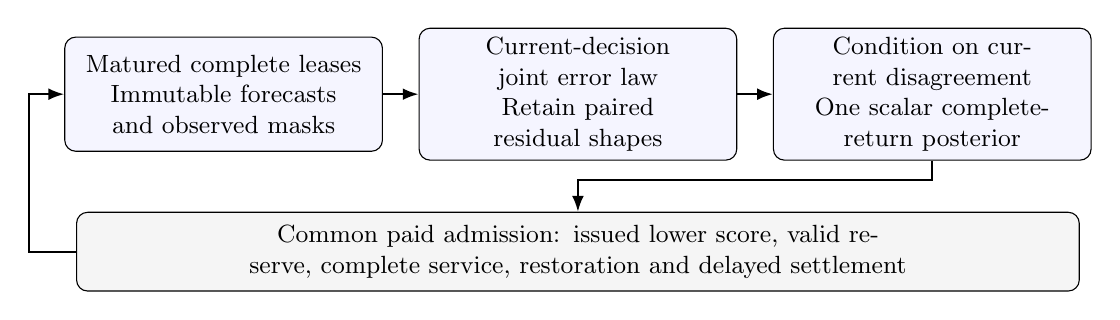
\begin{tikzpicture}[box/.style={draw,rounded corners,align=center,
text width=3.8cm,minimum height=1.45cm,font=\small,fill=blue!4},
flow/.style={-{Latex[length=2mm]},thick}]
\node[box] (history) at (0,0) {Matured complete leases\\Immutable forecasts and observed masks};
\node[box] (law) at (4.5,0) {Current-decision joint error law\\Retain paired residual shapes};
\node[box] (target) at (9,0) {Condition on current disagreement\\One scalar complete-return posterior};
\node[draw,rounded corners,align=center,font=\small,text width=12.5cm,
fill=gray!8,minimum height=1cm] (service) at (4.5,-2)
{Common paid admission: issued lower score, valid reserve, complete service, restoration and delayed settlement};
\draw[flow] (history)--(law);\draw[flow] (law)--(target);
\draw[flow] (target.south)--++(0,-.25)-|(service.north);
\draw[flow] (service.west)--++(-.6,0)|-(history.west);
\end{tikzpicture}}
\caption{One joint information-to-target mechanism. Historical masks remain
explicit; missing coordinates are integrated under a declared working law.
Current disagreement is available before future labels. The same service
contract and loss ledger execute CJ and every comparison method.}
\label{fig:conditional-overview}
\end{figure}

\subsection{A complete paid target shared by all sources}
At eligible origin $k$, source $s$ issues probabilities $p_{k,r,s}$ for
request $r$. Candidate and updating-reference classifiers $c_k^+,c_k^0$
remain fixed throughout a nonoverlapping lease of $H=4$ existing windows,
each containing at most 32 requests. Define
\begin{equation}
 b_k(x)=e_{c_k^+(x)}-e_{c_k^0(x)},\qquad
 h_{k,s}=\frac1{n_k}\sum_{r\in\mathcal O_k}
 p_{k,r,s}^{\mathsf T}b_k(x_r),\qquad N_k=Hn_k.
 \label{eq:current-contrast}
\end{equation}
The sources estimate the value of the same prepared candidate; they do not
create different deployed classifiers. $N_k$ is the origin-based service
capacity used to normalize the complete contrast. A short last window
retains all available requests and does not change actual accounting.
Unit utility per correct served request is used in the reported runs.

Let $g_k$ be the complete candidate/reference correctness contrast on
positions remaining after common model-work interruptions. Installation
and restoration cost three units. Admission additionally drops at most
two origin requests, with lost candidate correctness $\ell_k\in[0,2]$:
\begin{equation}
 U_k=g_k/N_k\in[-1,1],\qquad
 D_k=g_k-\ell_k-3=(g_k-5)+\delta_k,\quad
 \delta_k=2-\ell_k\in[0,2].
 \label{eq:complete-lease-return}
\end{equation}
$D_k$ includes the complete service effect and paid restoration.
Common preparation and reference-refresh fees are charged to every arm.
Forecast unavailability removes a forecast channel, rather than the
candidate's physical covariates, in the current replay contract.

Historical episode $j$ retains its immutable origin probabilities,
covariates, observed-source set $\mathcal S_j$ and complete label-maturity
time. Only nonempty blocks whose entire lease feedback has arrived are
eligible. Reproject them using the current candidate/reference:
\begin{equation}
 z_{j,s}^{(k)}=h_{j,s}^{(k)}-g_j^{(k)}/N_j,
 \qquad s\in\mathcal S_j.
 \label{eq:complete-joint-error}
\end{equation}
The complete target is recomputed with the current fixed versions on the
historical covariates and arrived labels. An unavailable historical source
remains unobserved. Neither a delayed outcome nor a repeated origin
forecast is counted as a new independent temporal observation.

The archive first retains the latest 48 complete matured lease records;
relevance and support filtering then determine which of these records
contribute. The contributing blocks receive the shared weights
\begin{equation}
 a_{j,k}=\beta^{k-j}
 \exp\{-\|x_k^{\rm ctx}-x_j^{\rm ctx}\|^2/\sigma_x^2\}\,d_{j,k},
 \qquad
 d_{j,k}=\frac{\#\{\text{lease requests with }c_k^+\ne c_k^0\}}
 {\#\{\text{lease requests}\}}.
 \label{eq:supported-history-kernel}
\end{equation}
Here $\beta=0.97$, $\sigma_x=3$ and weights below $10^{-12}$ are
excluded. Context comprises standardized source-group covariate means;
it does not include the current forecast disagreement. The support factor
uses covariates and current predictions, not the historical labels.

\subsection{A masked joint error law with retained pairing}
Let $H_j$ select the actually observed historical coordinates. Compute
$R_k\succ0$ from jointly observed full-source blocks, with prior mass
two, prior variance $0.01I$ and eigenvalue floor $10^{-6}$:
\begin{equation}
\begin{aligned}
 A_k&=2+\sum_{j:\mathcal S_j=\{1,\ldots,m\}}a_{j,k},\quad
 \bar z_k=A_k^{-1}\sum_{j:\mathcal S_j=\{1,\ldots,m\}}a_{j,k}z_j^{(k)},\\
 R_k&=\operatorname{floor}_{10^{-6}}\left[
 \frac{0.02I+\sum_{j:\mathcal S_j=\{1,\ldots,m\}}
 a_{j,k}z_j^{(k)}z_j^{(k)\mathsf T}}{A_k}
 -\bar z_k\bar z_k^{\mathsf T}\right].
\end{aligned}
\label{eq:predictive-joint-noise}
\end{equation}
Incompatible pairwise record sets are not assembled into a joint matrix.
For disjoint held-out prefix records $\mathcal I_0$, source quality is
$q_s=[|\mathcal I_0|^{-1}\sum_{i\in\mathcal I_0}
\|p_{i,s}-e_{y_i}\|_2^2+0.05]^{-1}$. Write $\bar q=m^{-1}\sum_sq_s$
and $P_{0,k}=0.01\diag(\bar q/q_s)$. The common location state is
\begin{equation}
\begin{aligned}
 P_k&=\left[P_{0,k}^{-1}+\sum_j a_{j,k}H_j^{\mathsf T}
 (H_jR_kH_j^{\mathsf T})^{-1}H_j\right]^{-1},\\
 \mu_k&=P_k\sum_j a_{j,k}H_j^{\mathsf T}
 (H_jR_kH_j^{\mathsf T})^{-1}z_j^{(k)}.
\end{aligned}
\label{eq:masked-precision-posterior}
\end{equation}
This is Gaussian power-likelihood conditioning, equivalently penalized
GLS. Every matrix comparator receives this same location unless its
explicit intervention factorizes the conditioning itself.

For each observed block, integrate missing coordinates using the Gaussian
Schur law, written in all-source coordinates:
\begin{equation}
 m_j=\mu_k+R_kH_j^{\mathsf T}R_{j,OO}^{-1}
       (z_j^{(k)}-H_j\mu_k),\qquad
 V_j=R_k-R_kH_j^{\mathsf T}R_{j,OO}^{-1}H_jR_k,
 \label{eq:masked-atoms}
\end{equation}
where $R_{j,OO}=H_jR_kH_j^{\mathsf T}$. The observed entries of $m_j$
remain the observed residuals. Missing coordinates and $V_j$ are working
conditional moments, not new observations. Add a zero-location prior atom
with covariance $R_k$ and mass two; normalize all masses to $\alpha_j$.
Center the atom locations $\bar m=\sum_j\alpha_jm_j$ and use
$\lambda_j=\mu_k+(m_j-\bar m)$ so that all information controls retain
the fitted mean correction $\mu_k$. Restrict to current active sources
only after constructing the historical law. Define
\begin{equation}
 f_{Z,k}(z)=\sum_j\alpha_j\phi_m(z;\lambda_j,\Sigma_j),\qquad
 \Sigma_j=V_j+P_k+b^2Q_k,\qquad
 Q_k=0.01\diag(\bar q/q_s).
 \label{eq:paired-error-law}
\end{equation}
Smoothing makes every component positive definite. Pairing is retained in
both the component locations and masked component covariance. Translation
and smoothing change the predictive law while leaving the archived
observations and masks unchanged. Error/target independence, Gaussian
missing-coordinate integration and weighted likelihoods are explicit
working assumptions, rather than automatic drift calibration.

\subsection{Conditioning the complete-error law on the current forecasts}
Let $Y_k=g_k/N_k$ be the normalized complete correctness contrast and
$Z_k=h_k-Y_k\mathbf1$ the complete source-error vector.  For any full-row-rank
$B\in\mathbb R^{(m-1)\times m}$ satisfying $B\mathbf1=0$, the current
forecast disagreement is an observed error contrast:
\begin{equation}
 BZ_k=Bh_k.
 \label{eq:conditional-disagreement-identity}
\end{equation}
Its availability does not depend on any future lease label.  The paired
law can therefore predict the common complete target by evaluating its
density on the line $h_k-u\mathbf1$ rather than reducing it to a covariance.
With the explicit working target prior $U\sim\operatorname{Unif}[-1,1]$
and error law independent of $U$ in the working generative model
$H=U\mathbf1+Z$, the scalar posterior is
\begin{equation}
 p_k(u\mid h_k)=
 \frac{\mathbf1_{[-1,1]}(u)f_{Z,k}(h_k-u\mathbf1)}
 {\int_{-1}^{1}f_{Z,k}(h_k-v\mathbf1)\,dv}.
 \label{eq:complete-target-line-posterior}
\end{equation}
The prior is part of the stated model; it is not a calibration claim.
The denominator must be positive and finite.  A positive definite smoothing
covariance makes this condition immediate for a Gaussian mixture.
The same prior, current forecasts, active-source set, matured archive,
fees, calibration protocol and execution rule apply to every control.

\paragraph{A single decision-relevant fusion functional.}
For $r=0,1,2$, write
\begin{equation}
 I_r(h;f)=\int_{-1}^{1}u^r f(h-u\mathbf1)\,du,\qquad
 \mathcal T(h;f)=
 \left(\frac{I_1}{I_0},
       \frac{I_2}{I_0}-\left(\frac{I_1}{I_0}\right)^2\right).
 \label{eq:decision-line-functional}
\end{equation}
The complete-target mean and variance are exactly $\mathcal T$.
All retained cross-source information reaches execution through this
one functional; intermediate locations, masked completion and smoothing
construct its input law rather than independently issuing actions.

\begin{proposition}[Decision sufficiency after joint conditioning]
\label{prop:line-functional-sufficiency}
Fix the current active mask, forecasts, capacity $N$, variance floor,
ready state, issued $q$ and pre-admission ledger. If two fitted laws have
the same $\mathcal T(h;f)$, they issue identical $F,S,L$, proposals and
guarded actions. Equality of unconditional residual coordinate marginals,
or of residual means and covariances, is insufficient in general when
multiple sources are active.
\end{proposition}
\begin{proof}
Insert Eq.~\eqref{eq:decision-line-functional} into
$F=N\mu$, $S=N\sqrt{v+\nu^2}$ and $L=F-qS-5$; the common gate and
ledger then give the same action. For insufficiency, the paired parity
laws in Eq.~\eqref{eq:conditional-parity-laws} have identical coordinate
marginals and full mean/covariance, while conditioning at the same
$h=c\mathbf1$ gives target means $c-a$ and $c+a$, both strictly inside
$(-1,1)$ for the displayed $c=5/128$ and $a=3/32$. Convolve both laws
with the same isotropic Gaussian of variance $\epsilon^2$. Their
coordinate marginals and full moments remain identical. As
$\epsilon\downarrow0$, the two target means converge to $c-a$ and
$c+a$: the nonconstant-sign atoms have strictly positive distance from
the conditioning line and their likelihood mass vanishes. With common
$q=0$, sufficiently small positive $\epsilon$ retains the opposite
paid proposals in Eq.~\eqref{eq:conditional-parity-paid-separation}.
Set common readiness to true and allow the same valid reservation in the
common ledger; these opposite proposals then produce opposite guarded actions.
\end{proof}
Thus a compact representation \emph{after} conditioning is exact for the
gate; preserving only residual summaries \emph{before} conditioning can
remove information needed to compute it. An estimator reproducing the
same conditional functional can reproduce CJ's actions. The contribution
concerns this information distinction and its measured paid value.

Each mixture component has a closed scalar representation.  Define
\begin{align}
 a_j&=\mathbf1^{\mathsf T}\Sigma_j^{-1}\mathbf1,
 & r_j&=\mathbf1^{\mathsf T}\Sigma_j^{-1}(h_k-\lambda_j),\nonumber\\
 \eta_j&=r_j/a_j,
 & s_j^2&=1/a_j,\nonumber\\
 c_j&=(h_k-\lambda_j)^{\mathsf T}\Sigma_j^{-1}(h_k-\lambda_j)-r_j^2/a_j.
 \label{eq:conditional-gaussian-line-components}
\end{align}
The conditional component is $\mathcal N(\eta_j,s_j^2)$ truncated to
$[-1,1]$.  Its mixture weight is proportional to
\begin{equation}
 \alpha_j|\Sigma_j|^{-1/2}e^{-c_j/2}a_j^{-1/2}
 \left[\Phi\left(\frac{1-\eta_j}{s_j}\right)
       -\Phi\left(\frac{-1-\eta_j}{s_j}\right)\right].
 \label{eq:conditional-gaussian-line-weights}
\end{equation}
This integrates the complete density, including its component-specific
normalization.  Normalizing only a likelihood at the closest point of
the line would omit the factor $a_j^{-1/2}$ and change the posterior.
The primary complete-value rule can take
$F_k=N_k\mathbb E[U\mid h_k]$ and
$S_k=N_k\sqrt{\operatorname{Var}(U\mid h_k)+\nu^2}$ and use the common score
$F_k-q_kS_k-5$.

\begin{proposition}[Coherent conditioning removes artificial source-weight gains]
\label{prop:conditional-simplex-invariance}
Set $c=m^{-1}\mathbf1^{\mathsf T}h$ and
$A=m^{-1}\mathbf1^{\mathsf T}Z$.  Conditional on $BZ=Bh$, one has
$Z=h+(A-c)\mathbf1$.  Consequently, for every simplex weight $w$,
\begin{align}
 w^{\mathsf T}h-\mathbb E[w^{\mathsf T}Z\mid Bh]&=
 c-\mathbb E[A\mid Bh],\nonumber\\
 w^{\mathsf T}h-\frac1t\log\mathbb E[e^{t w^{\mathsf T}Z}\mid Bh]
 &=c-\frac1t\log\mathbb E[e^{tA}\mid Bh].
 \label{eq:conditional-simplex-invariance}
\end{align}
The same identities hold after the target-prior truncation in
Eq.~\eqref{eq:complete-target-line-posterior}.  The scalar target law,
not an extra optimizer over source weights, supplies the increment.
\end{proposition}
\begin{proof}
$B(Z-h)=0$ and $\ker B=\operatorname{span}(\mathbf1)$ imply the stated
affine representation.  Substitute it and use $w^{\mathsf T}\mathbf1=1$.
The truncation restricts $A$ to $[c-1,c+1]$ without changing this identity.
\end{proof}
An untruncated Gaussian line posterior has mean
$\mathbf1^{\mathsf T}\Sigma^{-1}(h-m)/
(\mathbf1^{\mathsf T}\Sigma^{-1}\mathbf1)$ and variance
$(\mathbf1^{\mathsf T}\Sigma^{-1}\mathbf1)^{-1}$.
Its mean is exactly the generalized least-squares common-target estimate;
this provides a full-matrix deterministic control.  Truncation gives the
corresponding scalar truncated-normal posterior, rather than a distinct
information source.

\paragraph{A realizable separation from exact marginals and every pair law.}
Let $N=128$, $a=3/32$ and consider the two equal-mass error laws
\begin{equation}
\begin{aligned}
 \mathcal Z_+/a&=\{(+,+,+),(+,-,-),(-,+,-),(-,-,+)\},\\
 \mathcal Z_-/a&=\{(-,-,-),(-,+,+),(+,-,+),(+,+,-)\}.
\end{aligned}
\label{eq:conditional-parity-laws}
\end{equation}
They have identical source marginals, identical every-pair distributions,
mean zero, covariance $a^2I$ and atom radius.  Draw a regime
$\Theta\in\{+,-\}$ with equal probability, draw $Z$ from its error law,
draw $U$ independently from a common feasible bounded target prior, and issue
$H=U\mathbf1+Z$.  This generative model enforces $Z=H-U\mathbf1$;
the future outcomes are tied to the same law that generates the forecasts.
For example, take a discrete uniform prior over $NU\in\{-64,\ldots,64\}$.
All resulting source forecasts belong to $[-0.59375,0.59375]$.
The fitted uniform $[-1,1]$ prior is an explicit working choice; both
compatible target atoms below also lie inside that prior's support.

At $h=c\mathbf1$ with both $c-a$ and $c+a$ in the discrete prior's support
and inside its enclosing interval, zero disagreement
selects only $Z=+a\mathbf1$ under the plus regime and
$Z=-a\mathbf1$ under the minus regime.  Thus the complete-target posteriors
are respectively $U=c-a$ and $U=c+a$.  For $c=5/N$ and admissible
$\ell=2$, the complete returns are
\begin{equation}
 D_+=N(c-a)-5=-12,\qquad D_-=N(c+a)-5=12.
 \label{eq:conditional-parity-paid-separation}
\end{equation}
The exact joint law rejects the harmful case and admits the beneficial case.
Every controller retaining only the common coordinate marginals, pairwise
laws or first and second moments, along with the same current $h$, must
issue the same action in the two cases.  The two gross contrasts are
$g_+=-7$ and $g_-=17$, both realizable with binary labels and agreement
positions on a 128-request lease.  Source probabilities
$((1+h_s)/2,(1-h_s)/2)$ are valid because all displayed forecasts lie in
$[-1,1]$.  Historical projections $h_j=z_j$ with zero complete contrast
realize the archived errors.

The numerical check additionally realizes the declared chronology, outage
and support kernel: at current origin 240 it uses 32 fully observed matured
origins outside the two-window/13-window outage positions, within the last
48 potential four-window origins.  Each pattern occurs eight times.  Shared
label-free context distances attenuate the $\beta=0.97$ age weights and
$126/128$ disagreement support so that every pattern has effective mass
$1.5$, for total mass six.  Other potential origins have zero contrast support.
The prior mass is two with variance $0.01I$, correction prior $0.01I$,
and bandwidth $b=0.25$,
$Q=0.01I$, $q=1.2815515655$ and $\nu=0.01$.  The paired scalar posterior
and common $F-qS-5$ gate give scores $-18.212062$ and $+1.069772$,
while the exact product-of-marginals
and moment-matched full-Gaussian posteriors coincide across regimes.
The corresponding reduced scores are $-15.266708$ and $-9.980616$,
respectively.  A Gaussian-copula control with the exact marginals and
the matched correlation matrix is identical to the product control in
this example, because that correlation matrix is $I$.
The check calls the unchanged conditional implementation and independent
request-level service reconstructor.  It verifies all 32 historical projections
and zero gross targets, current gross targets $-7$ and $17$, two lost
candidate-correct requests, restoration, and complete returns $-12$ and $12$.
The common Fixed130/$B=130$ guard executes the beneficial case and rejects
the harmful case, with actual increments $12$ and zero.  The admitted
service-prefix minimum is $-2$ and the reconstruction error is zero.
This is a mechanism construction, not physical-stream performance evidence.

\paragraph{Standard value of information for complete paid return.}
The next statement is the binary-action specialization of the classical
value-of-information principle \cite{blackwell1953}; its application here
identifies exactly which expectation and execution conditions are needed.
Let $D$ be an integrable complete counterfactual return of the same fixed
candidate/reference lease.  Let $\mathcal R\subseteq\mathcal I$ be reduced
and retained information, each containing the current forecasts and common
execution state.  Let $G\in\{0,1\}$ be a common
$\mathcal R$-measurable indicator that this lease may execute with available
reserve.  Among measurable admission probabilities $0\leq A\leq G$, define
$V(\mathcal H)=\sup_A\mathbb E[AD]$.  Then
\begin{equation}
 V(\mathcal I)=\mathbb E[G(\mathbb E[D\mid\mathcal I])_+]
 \ \geq\ 
 \mathbb E[G(\mathbb E[D\mid\mathcal R])_+]=V(\mathcal R).
 \label{eq:conditional-complete-value-envelope}
\end{equation}
Writing $M=\mathbb E[D\mid\mathcal I]$, the exact gap is
\begin{equation}
 V(\mathcal I)-V(\mathcal R)=
 \mathbb E\left[G\min\left\{
 \mathbb E[M_+\mid\mathcal R],
 \mathbb E[(-M)_+\mid\mathcal R]\right\}\right].
 \label{eq:conditional-complete-value-strictness}
\end{equation}
It is strict precisely when the available reduced state has positive
conditional mass of retained conditional mean returns on both sides of zero.
\begin{proof}
For $\mathcal H$-measurable $A$,
$\mathbb E[AD]=\mathbb E[A\mathbb E[D\mid\mathcal H]]$.
The maximizing admission is $G\mathbf1_{\{\mathbb E[D\mid\mathcal H]>0\}}$.
The tower property and conditional Jensen inequality prove the inequality.
If $p=\mathbb E[M_+\mid\mathcal R]$ and
$n=\mathbb E[(-M)_+\mid\mathcal R]$, then
$\mathbb E[M\mid\mathcal R]=p-n$ and
$p-(p-n)_+=\min(p,n)$, proving the gap and strictness criterion.
\end{proof}
In Eq.~\eqref{eq:conditional-parity-paid-separation}, retained conditional
means are $-12$ and $12$ under the same reduced state, hence its conditional
value gap is six units.  A discrete uniform target prior over the feasible
integer gross contrasts gives a finite positive-probability construction;
the accompanying enumeration verifies a strict expected value gap over the
whole generative experiment.

This statement concerns optimal decisions under the true joint law (or the
explicit self-consistent construction).  Merely retaining a larger empirical
archive does not make its fitted posterior equal the physical conditional
law.  The subtraction $qS$ is conservative relative to the same fitted
mean $F$, rather than necessarily relative to the true-law optimizer.
The fitted gate need not attain its value; estimated calibration, drift and misspecification
can reverse a replay comparison.  The theorem establishes neither arbitrary
real-stream superiority nor conditional score coverage.  The same complete
return, same opportunities and same available reserve are essential.  If a
sequential budget binds, adding single-origin gaps is invalid: the full optimal
control problem can still emulate a reduced-information feasible policy, but
strict improvement requires a feasible action difference after accounting for
future reserve use.  The existing execution-loss budget remains a separate
pathwise statement shared by all posterior choices.

\paragraph{When retained information survives the fitted paid gate.}
Fix one candidate/reference lease with integrable complete return $D$ and
reduced and retained information $\mathcal R\subseteq\mathcal I$.
Both contain the same current forecasts, model versions and prefix execution
state.  Require common readiness and the same settled loss $C_t$, unresolved
reserve $Q_t$ and proposed reserve $M_k$.  Thus the common indicator
\begin{equation}
 G=\mathbf1\{\text{ready}\}\mathbf1\{C_t+Q_t+M_k\leq B\}
 \label{eq:final-paid-common-feasibility}
\end{equation}
is $\mathcal R$-measurable.  All expectations below concern the true physical
joint law, or an explicitly self-consistent generative construction, at this
common state.  For $\mathcal H\in\{\mathcal R,\mathcal I\}$, put
$m_{\mathcal H}=\mathbb E[D\mid\mathcal H]$ and
$V(\mathcal H)=\mathbb E[G(m_{\mathcal H})_+]$.
The binary-action information gap is
\begin{equation}
 \Delta=V(\mathcal I)-V(\mathcal R)
 =\mathbb E\!\left[G\min\!\left\{
 \mathbb E[(m_{\mathcal I})_+\mid\mathcal R],
 \mathbb E[(-m_{\mathcal I})_+\mid\mathcal R]\right\}\right]\geq0.
 \label{eq:final-paid-information-gap}
\end{equation}
Consequently, a positive gap requires feasible reduced states in which the
retained conditional paid mean falls on both sides of zero with positive
conditional probability.  A change in a fitted covariance or posterior
alone does not establish such a gap.

\begin{proposition}[Fitted paid-action regret and sufficient benefit]
\label{prop:final-fitted-paid-benefit}
Let $F_{\mathcal H},S_{\mathcal H},q_{\mathcal H}$ be issuance-time
$\mathcal H$-measurable quantities, with
$r_{\mathcal H}=q_{\mathcal H}S_{\mathcal H}\geq0$ and
$\widehat m_{\mathcal H}=F_{\mathcal H}-5$.  Suppose the quantities below
are integrable and issue the same paid gate as the executable controller:
\begin{equation}
 L_{\mathcal H}=\widehat m_{\mathcal H}-r_{\mathcal H},\qquad
 A_{\mathcal H}=G\mathbf1\{L_{\mathcal H}>0\}.
 \label{eq:final-fitted-paid-gate}
\end{equation}
Its exact regret and bound are
\begin{align}
 \operatorname{Reg}_{\mathcal H}
 &:=V(\mathcal H)-\mathbb E[A_{\mathcal H}D]\nonumber\\
 &=\mathbb E\!\left[G|m_{\mathcal H}|\mathbf1\left\{
 \mathbf1\{L_{\mathcal H}>0\}\ne\mathbf1\{m_{\mathcal H}>0\}
 \right\}\right]\nonumber\\
 &\leq\underbrace{\mathbb E[G|\widehat m_{\mathcal H}-m_{\mathcal H}|]}
                 _{\varepsilon_{\mathcal H}}
       +\underbrace{\mathbb E[Gr_{\mathcal H}]}_{\rho_{\mathcal H}}.
 \label{eq:final-fitted-paid-regret}
\end{align}
Against every $\mathcal R$-measurable admission probability
$0\leq A_{\mathcal R}\leq G$, the fitted retained gate satisfies
\begin{equation}
 \mathbb E[(A_{\mathcal I}-A_{\mathcal R})D]
 \geq\Delta-\varepsilon_{\mathcal I}-\rho_{\mathcal I}.
 \label{eq:final-fitted-paid-improvement}
\end{equation}
In particular, $\Delta>\varepsilon_{\mathcal I}+\rho_{\mathcal I}$ is
sufficient for strictly greater expected complete paid return.
\end{proposition}
\begin{proof}
Condition on $\mathcal H$.  The oracle admits exactly when
$m_{\mathcal H}>0$; subtracting the fitted admission gives the exact
regret identity.  A harmful admission has
$m_{\mathcal H}\leq0<\widehat m_{\mathcal H}-r_{\mathcal H}$, hence
$|m_{\mathcal H}|\leq|\widehat m_{\mathcal H}-m_{\mathcal H}|$.
A missed benefit has
$m_{\mathcal H}>0\geq\widehat m_{\mathcal H}-r_{\mathcal H}$, hence
$m_{\mathcal H}\leq|\widehat m_{\mathcal H}-m_{\mathcal H}|+r_{\mathcal H}$.
Integrate, and use $\mathbb E[A_{\mathcal R}D]\leq V(\mathcal R)$.
\end{proof}

For CJ, $F=N\widehat\mu$ and
$S=N\sqrt{\widehat v+\nu^2}$ are moments of the fitted bounded working
posterior.  With $D=NU-5+\delta$, the paid-mean error explicitly includes
the service slack:
\begin{equation}
 \varepsilon_{\mathcal I}
 \leq\mathbb E\!\left[GN
     |\widehat\mu-\mathbb E[U\mid\mathcal I]|\right]
     +\mathbb E[G\delta],\qquad \delta=2-\ell\geq0.
 \label{eq:final-paid-target-error}
\end{equation}
Thus retained pairing supplies possible oracle value; physical estimation
error and the issued $qS$ penalty can consume it.  Distances between fitted
information controls do not bound $\varepsilon_{\mathcal I}$ without a
separate physical estimation guarantee.  The result promises neither
larger admission counts nor conditional coverage for accepted leases.

The common-state restriction is essential.  Different earlier actions can
change $C_t,Q_t$, later feasibility and the delayed $q$ states.  One cannot
sum these single-origin gaps across separately evolving ledgers.  A
sequential comparison requires the full continuation value of feasible
policies, or explicit coupling that keeps the compared execution state
identical.  The shared pathwise loss-budget theorem remains independent of
this expected information benefit.

\paragraph{A controlled bridge from retained pairing to the paid gate.}
Let $f_0,f_1$ be two residual densities evaluated with the same active
sources, current forecast $h$, bounded target prior and execution state.
For $0\leq\tau\leq1$, define $f_\tau=(1-\tau)f_0+\tau f_1$.
For $f_0=f_{\mathrm M}=\prod_s f_{\mathrm J,s}$ and
$f_1=f_{\mathrm J}$, every coordinate marginal is identical for all $\tau$.
Applying the same replacement $P\mapsto\operatorname{diag}P$ in both
endpoints preserves those marginals and removes the contribution of the
off-diagonal correction covariance while retaining historical atom pairing.
A second bridge uses the full Gaussian $f_{\mathrm G}$ matching the paired
law's residual mean and covariance as $f_0$.  Its residual mean and full
covariance are identical for all $\tau$, so any response to this bridge
comes from distributional shape beyond those moments.  These are controlled
changes to the retained law. The executed primary algorithm remains the
full paired endpoint $\tau=1$; $\tau$ is an information intervention,
not an additional fitted parameter or execution component.

\begin{proposition}[Retained-law bridge and paid-score stability]
\label{prop:retained-pairing-paid-bridge}
Write $e_r(h)=\int_{-1}^{1}f_r(h-u\mathbf1)\,du\in(0,\infty)$ and
let $p_r$, $\mu_r$ and $v_r$ be its normalized scalar target posterior,
mean and variance, for $r\in\{0,1\}$.  Then
\begin{align}
 \rho_\tau(h)&=\frac{\tau e_1(h)}{(1-\tau)e_0(h)+\tau e_1(h)},
 &p_\tau&=(1-\rho_\tau)p_0+\rho_\tau p_1,
 \label{eq:retained-bridge-posterior}\\
 \mu_\tau&=\mu_0+\rho_\tau d,
 &v_\tau&=v_0+\rho_\tau(v_1-v_0)+\rho_\tau(1-\rho_\tau)d^2,
 \qquad d=\mu_1-\mu_0.
 \label{eq:retained-bridge-moments}
\end{align}
In particular, $\operatorname{TV}(p_\tau,p_0)=
\rho_\tau\operatorname{TV}(p_1,p_0)$.
For the common paid score $C_\tau=N\mu_\tau-qN\sqrt{v_\tau+\nu^2}-5$,
where $N>0$, $q\geq0$ and $\nu>0$ are fixed, the exact score change is
\begin{equation}
 C_\tau-C_0=N\rho_\tau d-qN
 \left[\sqrt{v_\tau+\nu^2}-\sqrt{v_0+\nu^2}\right].
 \label{eq:retained-bridge-paid-score}
\end{equation}
Its local response is
\begin{equation}
 \frac{dC_\tau}{d\tau}=N\rho'_\tau
 \left[d-\frac{q\{v_1-v_0+(1-2\rho_\tau)d^2\}}
 {2\sqrt{v_\tau+\nu^2}}\right],\qquad
 \rho'_\tau=\frac{e_0e_1}{\{(1-\tau)e_0+\tau e_1\}^2}>0.
 \label{eq:retained-bridge-score-response}
\end{equation}
At a commonly ready and feasible origin the retained law changes rejection into
admission exactly when $C_0\leq0<C_1$.  In particular,
$\mu_1\geq\mu_0$ and $v_1\leq v_0$ imply $C_1\geq C_0$; the endpoint
inequality is strict if $\mu_1>\mu_0$, or if $q>0$ and $v_1<v_0$.

More generally, if $\delta=\operatorname{TV}(p_0,p_1)$, with TV defined
as one half of the $L^1$ distance, and $b_\delta=\min\{1,4\delta\}$, then
\begin{align}
 |F_1-F_0|&\leq2N\delta,
 &|v_1-v_0|&\leq b_\delta,\nonumber\\
 |C_1-C_0|&\leq K_\delta
 :=N\left[2\delta+q\{\sqrt{\nu^2+b_\delta}-\nu\}\right].
 \label{eq:retained-bridge-score-tv}
\end{align}
Thus $C_0>K_\delta$ protects admission and $C_0<-K_\delta$ protects
rejection under this perturbation, given the same execution state.
\end{proposition}
\begin{proof}
Normalization of the affine likelihood gives
Eq.~\eqref{eq:retained-bridge-posterior}; the laws of total expectation
and total variance give Eq.~\eqref{eq:retained-bridge-moments}.
Substitution and differentiation give the score identities.
Coordinate integration proves the marginal assertion.  If both residual
endpoints have mean $m$ and covariance $\Sigma$, their affine density
mixture has the same first and second moments, proving the Gaussian-bridge
assertion.  For any bounded function $a$, the TV inequality is
$|\mathbb E_1a-\mathbb E_0a|\leq(\sup a-\inf a)\delta$.
Apply it to $a(u)=u$ for the mean bound.  Since
$v_r=\min_{t\in[-1,1]}\mathbb E_r[(U-t)^2]$, evaluate the other law
at the minimizing $t$ of the smaller-variance law.  The squared-loss range
is at most four, giving $|v_1-v_0|\leq4\delta$; also $0\leq v_r\leq1$.
For $x,y\geq0$ with $|x-y|\leq b_\delta$, concavity gives
$|\sqrt{x+\nu^2}-\sqrt{y+\nu^2}|\leq\sqrt{\nu^2+b_\delta}-\nu$.
Combine the bounds with the common score and its strict positive gate.
\end{proof}

The between-posterior term in Eq.~\eqref{eq:retained-bridge-moments}
is essential: mixing two concentrated but separated target laws can increase
uncertainty.  The bridge therefore supplies an exact diagnostic of how
retained pairing changes a paid action, not a monotone benefit guarantee.
Its moment-to-score expressions apply to ready origins; the common reference
fallback at an unready origin remains unchanged.
Its score margin protects a decision against a specified posterior change;
complete executed return still requires the action and service accounting.
Computable TV between fitted endpoints measures sensitivity to the declared
information reduction.  It does not bound TV to the unknown physical
conditional law without an additional estimation or calibration guarantee.

\subsection{One paid score, delayed feedback and exact return}
The executable proposal uses the complete-target moments,
\begin{equation}
 F_k=N_k\mathbb E[U\mid h_k],\qquad
 S_k=N_k\sqrt{\operatorname{Var}(U\mid h_k)+\nu^2},\qquad
 L_k=F_k-q_kS_k-5,\quad \widetilde a_k=\mathbf1\{L_k>0\},
 \label{eq:posterior-gate}
\end{equation}
with $\nu=0.01$. The evaluated interface requires at least one active
forecast source. With no eligible error evidence, $F_k=0$ retains the
reference. Singleton masks use the same scalar target posterior. For CJ,
the mixture's truncated-normal target moments are analytic; no source-weight
optimizer is executed. The legacy source-weight field contains fixed quality
weights only and influences neither $F_k$ nor admission.

Save the issued $F_k,S_k,q_k$. At complete outcome maturity, set
$T_k=(F_k-g_k)/S_k$, $v_k=\mathbf1\{T_k>q_k\}$ and perform
\begin{equation}
 q^+=\max\{q_{\min},q+0.05(v_k-0.1)\}.
 \label{eq:delayed-calibration-update}
\end{equation}
Rejected eligible episodes also receive callbacks. Only mature, ready
first-half calibration forks initialize $q_0$ using the higher 90th
percentile of issued pilot errors, clipped below at $q_{\min}$; an empty
set uses $q_{\min}$. Second-half complete paid return selects the declared
configuration. Adaptive miscoverage feedback follows \cite{gibbs2021}.
If $r_u=q^+-q-0.05(v_{j_u}-0.1)\geq0$, the exact update identity is
\begin{equation}
 \sum_{u=1}^{M}v_{j_u}
 =0.1M+\frac{q_M-q_0-\sum_{u=1}^{M}r_u}{0.05}.
 \label{eq:delayed-calibration-accounting}
\end{equation}
Pending callbacks remain pending. The identity is not a finite-sample
accepted-action coverage theorem.

\begin{theorem}[Complete paid return and changed-action accounting]
\label{thm:paid-return}
Under the fixed-version, nonoverlapping lease contract with restoration,
a covered proposal $T_k\leq q_k$ satisfies $D_k\geq L_k$.
Every completed trajectory obeys
\begin{equation}
\begin{aligned}
 J-J^0&=\sum_k a_kD_k,\qquad
 D_k=L_k-S_k(T_k-q_k)+\delta_k,\\
 J-J^0&\geq\sum_k a_kL_k-\sum_k a_kS_k(T_k-q_k)_+.
\end{aligned}
\label{eq:weighted-return-bound}
\end{equation}
For controllers $F,C$ with the same model versions, targets and common-work
costs, define $\mathcal I_{10}=\{k:a_k^F=1,a_k^C=0\}$ and
$\mathcal I_{01}=\{k:a_k^F=0,a_k^C=1\}$. Then
\begin{equation}
\begin{aligned}
 J_F-J_C={}&\underbrace{\sum_{\mathcal I_{10}}(D_k)_+}_{\text{additional gain}}
 +\underbrace{\sum_{\mathcal I_{01}}(-D_k)_+}_{\text{avoided loss}}\\
 &-\underbrace{\sum_{\mathcal I_{01}}(D_k)_+}_{\text{missed gain}}
 -\underbrace{\sum_{\mathcal I_{10}}(-D_k)_+}_{\text{incurred loss}}.
\end{aligned}
\label{eq:action-gain-decomposition}
\end{equation}
\end{theorem}
\begin{proof}
Substitute $g_k=F_k-S_kT_k$ into
Eq.~\eqref{eq:complete-lease-return}. Nonnegative $\delta_k$ gives the
covered-score implication and replacing an excess by its positive part
gives the bound. Restoration and nonoverlap make complete service effects
additive. Common actions cancel; splitting each remaining return into
positive and negative parts proves the changed-action identity.
\end{proof}
This connects retained information to executed benefit, rather than
counting different matrices or weights as service gains. Coverage is tested
at informative origins and actual admissions, together with optimistic
excess $S_k(T_k-q_k)_+$ in complete-return units. Its weighted sum enters
Eq.~\eqref{eq:weighted-return-bound} directly.

\paragraph{The paid value of retained joint information.}
At an issuance state, keep the matured archive, current forecasts, quality,
candidate/reference versions, issued threshold and pre-action ledger fixed.
Let $b_{r,k}=\mathbf1\{F_{r,k}-q_kS_{r,k}-5>0\}$ for the retained law
$r=J$ and an information reduction $r=R$. Write $G_k$ for their common
readiness and reservation feasibility. The direct paid contribution is
\begin{equation}
 \Psi_{J:R}=\sum_kG_k(b_{J,k}-b_{R,k})D_k.
 \label{eq:paid-retained-information}
\end{equation}
This estimand isolates the information map. A whole-policy comparison also
allows calibration and the ledger to evolve, and is reported separately.

\begin{corollary}[Completed-target certificate for retained information]
\label{cor:paid-retained-information}
Let $\mathcal K_{10}$ and $\mathcal K_{01}$ be the commonly feasible
joint-only and reduction-only actions. Under the complete lease contract,
\begin{equation}
\begin{aligned}
 \Psi_{J:R}\geq{}&
 \sum_{k\in\mathcal K_{10}}\{L_{J,k}-S_{J,k}(T_{J,k}-q_k)\}\\
 &-\sum_{k\in\mathcal K_{01}}\{L_{R,k}-S_{R,k}(T_{R,k}-q_k)+2\}.
\end{aligned}
 \label{eq:paid-information-certificate}
\end{equation}
If $\mathcal K_{01}=\varnothing$, $\mathcal K_{10}\ne\varnothing$ and
$T_{J,k}\leq q_k$ on $\mathcal K_{10}$, then
$\Psi_{J:R}\geq\sum_{k\in\mathcal K_{10}}L_{J,k}>0$.
\end{corollary}
\begin{proof}
The complete-return identity gives
$D_k=L_{r,k}-S_{r,k}(T_{r,k}-q_k)+\delta_k$, with
$0\leq\delta_k\leq2$. A joint-only action contributes $D_k$, bounded
below by setting $\delta_k=0$; a reduction-only action contributes $-D_k$,
bounded below by setting $\delta_k=2$. Summing proves the bound.
Coverage and strict admission make the final lower sum positive.
\end{proof}
This is a complete-feedback accounting consequence of
Theorem~\ref{thm:paid-return}. It connects an isolated information change
to a paid return certificate; the issued controller still uses only
available information before outcomes arrive.

\subsection{A common pathwise loss guarantee}
Every controller uses the same permanent-loss ledger. Let $C_t$ be settled
negative return and $Q_t$ unresolved reserved liability:
\begin{equation}
 C_t=\sum_{j\in\mathcal M_t}(-D_j)_+,\qquad
 Q_t=\sum_{j\in\mathcal P_t}M_j,\qquad
 a_k=\widetilde a_k\mathbf1\{C_t+Q_t+M_k\leq B\}.
 \label{eq:loss-budget-gate}
\end{equation}
Profit does not refill spent loss. Immutable lease IDs, atomic admission
and settlement, and valid bounds for both complete loss and every adverse
service prefix are required. The tested common-work interruption removes
at least one origin request. A four-window lease has at most 127 positions after common interruptions.
After admission drops, at most 125 served contrast positions and two lost
reference positions contribute adverse return, with three paid units;
thus the valid fixed reserve is $M_k=130$. If an application changes that
contract, it must recompute the reserve.

\begin{theorem}[Shared unconditional execution-loss bound]
\label{thm:unconditional-loss-budget}
For arbitrary outcomes and feedback delays, including permanently missing
feedback, valid reserves and the enforced service contract imply
\begin{equation}
 C_t+Q_t\leq B,\qquad
 \sum_{j\in\mathcal A}(-D_j)_+\leq B,\qquad
 J(t)-J^0(t)\geq-B.
 \label{eq:pathwise-loss-budget}
\end{equation}
\end{theorem}
\begin{proof}
The admission test preserves $C_t+Q_t\leq B$. Settlement replaces $M_j$
by $(-D_j)_+\leq M_j$ and cannot increase liability; unresolved leases
retain their reserves. Each completed negative return is bounded by its
charged liability, and each open service-prefix effect by its reserve.
Additivity and induction prove all three inequalities.
\end{proof}
The guarantee is common to marginal, matrix, copula and neural controls.
It protects cumulative downside without promising positive return or
correct posterior calibration on every stream. At fixed $B=M$, one settled
negative lease makes subsequent fixed-$M$ reservations infeasible. Fusion's
independent benefit must therefore be measured using the same budget,
including useful proposals refused after liability has been spent.
Independent recording chains restart the ledger: ten such chains have
aggregate bound $10B$, not a single $B$ bound.

\subsection{Execution and numerical reproducibility}
The live interface accepts current source forecasts and IDs, fixed model
versions, complete matured error blocks, prefix quality, mature calibration
state and service feasibility. Forecast moments and paid decisions depend
on no current or future labels. The offline replay separately constructs
complete-truth callback and verification fields, releasing callbacks only
at complete maturity; those fields do not enter issuance or admission.
A production service computes the callback target after feedback arrives.
The order is: reproject complete arrived blocks; build the masked law;
evaluate its current-target line posterior; issue the score; atomically
reserve; serve and restore; settle when complete feedback arrives.
The posterior and callback logs preserve issuance-time quantities.
Missing forecast coordinates remain explicitly masked. Numerical
validation failures stop the evaluated replay and retain their diagnostics;
a live service must handle them before authorizing a deployment.

CJ integrates at most 49 components. Its dominant per-origin matrix
work is $O(Jm^3)$ for $J\leq49$; target moments are scalar analytic
calculations. Product and copula controls use composite Gauss--Legendre
integration with moment refinement checks; these tolerances do not bound
statistical error. The copula's normal-CDF approximation and tail clipping
are checked separately. Singleton and multi-source paths, chronological
label eligibility, and poisoning of offline truth fields are checked in
the supplied code. Runtime and hardware cost claims require separate
measurement; operation counts are not measured latency.

\section{Performance}
\label{sec:performance}

The evaluation follows retained joint information through the complete-target
posterior, issued admission, served requests and paid net return. On RSS,
CJ obtains 35.6 mean net units under the shared fixed-130 reserve and
130-unit permanent-loss budget, versus 16.8 for the exact-marginal,
factorized, full-Gaussian, block-sandwich and Gaussian-copula conditional
controls. It retains all nine beneficial leases admitted by each of these
controls and adds four more, increasing their pooled count from nine to
13. The four additional leases supply 106 correct-served utility units,
pay 12 extra installation/restoration units and deliver 94 net units,
or 18.8 per delay schedule. This is a directly reconstructed useful-action
contribution under the same execution guarantee.

\begin{table}[t]
\centering\small
\caption{Core paid value of retained joint information on RSS. The
comparison family is exact marginal, factorized, full Gaussian/GLS,
block sandwich and Gaussian copula. Counts pool the five shared delays;
four replay cases arise at two distinct physical origin windows.}
\label{tab:core-paid-pairing-value}
\begin{tabular}{p{.63\linewidth}r}
\toprule
Mechanism-to-service endpoint & Measured increment\\
\midrule
Beneficial admissions: matched controls $9$ to CJ $13$ & $+44.44\%$\\
Additional beneficial complete leases & $4$\\
Retained control-admitted beneficial leases & $9/9$\\
Covered completed targets among additional leases & $4/4$\\
Additional correctly served utility & $106$\\
Additional installation and restoration fees & $12$\\
\textbf{Additional complete paid net utility} & $\mathbf{94}$\\
\textbf{Mean net utility increment per delay} & $\mathbf{18.8}$\\
Completed-target interruption-robust lower bound & $92$\\
Covered issued-score lower bound & $1.7506752582$\\
\bottomrule
\end{tabular}
\end{table}

We also intervene continuously on retained pairing while preserving
coordinate marginals or full second-order moments. These fixed-state
analyses connect the amount of joint information to target inference and
executed return. RSS remains an inspected development trace. A separately
frozen four-tag physical collection and a subsequent dual-accelerometer
collection with ten unseen participants supply transfer and execution evidence;
all primary outcomes, stronger operational choices and calibration strata
remain reported with their corresponding evidence scope.

The endpoints are cost-inclusive utility, additional and missed beneficial
return, avoided and incurred negative return, admitted-score coverage and
optimistic excess. We distinguish theoretical identifiability, fixed-state
mechanism interventions, complete policy comparison and new physical
validation. These questions require different evidence; a valid information
construction or many reconstructed trajectories cannot by itself establish
cross-environment superiority.

\subsection{Physical evidence, service contract and development selection}
The inspected development traces are Indoor User Movement Prediction from
RSS Data, AReM and Gas sensors for home activity monitoring
\cite{rss348,arem366,gashome362}. They contain, respectively, four
receiver groups, three physical RSS links and the declared physical gas
sensor views. Their previously retained data adapters, participant/recording
splits and immutable forecast archives are unchanged. Every recorded
configuration and earlier selector remains in the reproduction package.
RSS records signals from four fixed anchors to a chest-worn mote at 8 Hz;
the two classes indicate room-changing or room-preserving trajectories.
The original collection has 13,197 rows and 314 trajectory files across
three office settings, each with two rooms and a corridor; anchors are
1.5 m above the floor and released signals are normalized per anchor to
$[-1,1]$ \cite{rss348}. These collection descriptors do not constitute
three newly held-out sites in the present ordered RSS replay.

\begin{table}[t]
\centering\small
\caption{Physical acquisition and executable service parameters. RSS
supplies the controlled pairing mechanism evidence; HARTH supplies the
previously frozen, disjoint-participant evaluation. Both use the same
four-window paid contract and permanent-loss guard.}
\label{tab:physical-service-parameters}
\begin{tabular}{p{.31\linewidth}p{.29\linewidth}p{.29\linewidth}}
\toprule
Parameter & RSS & HARTH\\
\midrule
Physical source groups & Four fixed RSS anchors & Lower-back/right-thigh accelerometers\\
Acquisition rate & 8 Hz & 50 Hz; stride-50 snapshots\\
Target & Two movement classes & Twelve activity classes\\
Physical test role & Known ordered trace & Ten disjoint held-out participants\\
Eligible lease origins & 42 per delay & 1,560 pooled across five delays\\
Lease and request utility & Four windows, at most 32 requests/window; one unit/correct request & Same contract\\
Installation/restoration & $2+1$ utility units & Same fees\\
Additional interruption & At most two origin requests & Same interruption rule\\
Delayed feedback & One--four windows & Same delay support\\
Forecast unavailability & Rotating source, first two of every 13 windows & Same forecast-only schedule\\
History and context & Last 48 matured leases, $\beta=0.97$, $\sigma_x=3$ & Same kernel and capacity\\
Reserve/loss budget & $M=130$, $B=130$ per chain & Same, reset per history run\\
\bottomrule
\end{tabular}
\end{table}

The new CJ selector maximizes calibration return and breaks ties by larger
feedback floor and then larger bandwidth. Greater smoothing is preferred
only when calibration cannot distinguish paid return. This rule was
fixed before the new physical collection was acquired.

All conditional controls receive nine configurations,
$b\in\{0.25,0.5,1\}$ and
$q_{\min}\in\{0,0.64,1.2815515655\}$, on the same three calibration
delay schedules. Initial quantiles use only ready first-half outcomes that
have fully matured at the calibration boundary. Second-half complete
lease return selects the controller. Five common delay schedules evaluate
each known trace. Source predictors and the shared candidate are linear
softmax models: learning rate 0.08, $L_2$ coefficient 0.003, 500 initial
gradient steps and 20 steps every four windows. After online feedback
arrives, work uses the latest 512 arrived, nonreserved training records.
The shared reference refreshes every eight windows.

Every method sees the same current $h$, quality, covariate context, kernel,
source masks, historical complete targets, label delays, candidate/reference
versions and paid lease. Labels have imposed delays of one to four windows;
forecast-only outages hide one rotating source during the first two of every
13 windows. These delays, outages and monetary-unit fees are controlled
replay interventions. A lease contains four available windows of at most
32 rows, including a short terminal window when present; it never crosses
a recording boundary in the new physical evaluation. Leases include
installation, interruption and restoration. Utility is independently
reconstructed from served requests and direct fees, rather than merely
summed from stored predicted gains.

\subsection{Strong information reductions and external neural fusion}
The primary comparison changes retained information inside the same
complete-target conditional rule:

\begin{table}[t]
\centering\small
\caption{Same-information conditional fusion controls. Every row observes
the current source disagreement and uses the same delayed gate and ledger.}
\label{tab:conditional-controls}
\begin{tabular}{p{.24\linewidth}p{.68\linewidth}}
\toprule
Controller & Information supplied to the complete-target line posterior\\
\midrule
CJ & Paired masked mixture with the common correction location.\\
Exact marginal & Product of the CJ law's exact coordinate mixture
marginals; same fitted location and marginal uncertainty.\\
Factorized & Diagonal working covariance before masked correction and
completion; product of the resulting coordinate marginals.\\
Full Gaussian / GLS & Exact CJ-law mean and full covariance, including
correction uncertainty; deterministic common-target GLS has the same
untruncated Gaussian mean.\\
Block sandwich & Full Gaussian with a same-history joint-block HC0
sandwich replacing the correction covariance.\\
Gaussian copula & Exact coordinate mixture densities plus an adaptive
latent Gaussian correlation matrix derived from the same total covariance.\\
CJ--diagonal $P$ & Retained joint atoms with $P$ replaced by $\diag(P)$;
coordinate marginals stay identical to the exact-marginal control.\\
\bottomrule
\end{tabular}
\end{table}

The exact-marginal arm does not discard current disagreement or the
jointly fitted mean. The copula retains non-Gaussian coordinate mixtures
and adaptive matrix dependence, making it a stronger reduction than
independence. Its latent correlation is the normalized total covariance;
a nonlinear marginal transform need not reproduce that covariance as a
physical Pearson covariance. Normal-CDF approximation error, clipping
at $10^{-12}$ and one-dimensional integration refinement are disclosed
separately. This is a designed Gaussian-copula reference, rather than an
original vine-copula reproduction. A deterministic method preserving the
entire conditional joint law can reproduce CJ; the information reduction,
rather than a Bayesian designation, defines these comparisons.

Published external methods are Predictive Dynamic Fusion (PDF)
\cite{pdf2024} and Quality-aware Multimodal Fusion (QMF)
\cite{qmf2023}. We include their nonlinear tabular adaptations with
one encoder per physical source, 32 tanh units, class heads and confidence
heads. Training activates the original PDF confidence/prediction objectives
and QMF quality/ranking objectives, rather than using only a frozen
confidence formula. Confidence-loss coefficients are 1.0 for PDF and 0.1
for QMF. The source implementations are bound to author-code commits
\texttt{864867426cde076f} and \texttt{fe6c4c6ef7cb23f0}.
The original image/text architectures and leaderboards are not reproduced.
These comparisons test published fusion objectives in the shared service
setting. They use the same candidate/reference versions and execution
contract; extra neural encoder work is disclosed and is not claimed to
have identical hardware cost to the linear source models.

On the four-tag UCI196 collection, each external rule receives the same nine-trial
budget: learning rates $\{0.02,0.08,0.2\}$ crossed with paid margins
$\{0,4,12\}$, evaluated on the same three calibration schedules and five
calibration recordings. Its scalar complete-error gate is separately
calibrated using the same chronology. Both external and all internal
selections are hash-locked before any held-out outcome replay.

\subsection{Joint structure changes useful RSS actions}
Table~\ref{tab:conditional-development} gives the cost-inclusive primary
operating point. All five RSS increments are nonnegative; the comparison
with each reduced conditional law improves in three schedules and ties
in two. The paired CJ-minus-control differences are $[28,38,0,28,0]$,
mean 18.8. The conditional five-delay $t_4$ interval is
$[-3.10,40.70]$; it describes imposed-delay variation on this inspected
trace and does not estimate site-level generalization.

\begin{table}[t]
\centering\small
\caption{Measured reference-relative mean net utility on known development
traces at fixed reserve 130 and $B=130$. RSS counts pool five shared
schedules; all complete outcomes, including zero and negative leases,
are retained.}
\label{tab:conditional-development}
\begin{tabular}{lrrrrrr}
\toprule
Controller & RSS & AReM & GasHome & RSS adm. & Beneficial & Harmful\\
\midrule
CJ & 35.6 & $-30.0$ & 45.2 & 16 & 13 & 1\\
Exact marginal & 16.8 & $-30.0$ & 45.2 & 12 & 9 & 1\\
Factorized & 16.8 & $-30.0$ & 45.2 & 12 & 9 & 1\\
Full Gaussian / GLS & 16.8 & $-30.0$ & 45.2 & 12 & 9 & 1\\
Block sandwich & 16.8 & $-30.0$ & 45.2 & 12 & 9 & 1\\
Gaussian copula & 16.8 & $-30.0$ & 45.2 & 12 & 9 & 1\\
CJ--diagonal $P$ & 35.6 & $-30.0$ & 45.2 & 16 & 13 & 1\\
\bottomrule
\end{tabular}
\end{table}

Against each exact-marginal, factorized, Gaussian, sandwich and copula
conditional controller, the executed RSS difference comprises four
additional beneficial actions totaling 94 units. All nine control-admitted
beneficial leases are retained; missed beneficial return and additional
negative return are both zero in this comparison. The beneficial-action
count increases by 44.44\%. Equation~\eqref{eq:action-gain-decomposition}
gives $94/5=18.8$ mean units. Both policies retain one $-1$ lease.
CJ--diagonal $P$ has the same actions as CJ, locating the observed gain
in the retained predictive pairing and conditional target law.

For the four changed leases, the shared three-unit action fee permits
the exact service decomposition
\begin{equation}
 \Delta C^{\rm served}=\sum_{k\in\mathcal I_{10}}(D_k+3)=106,
 \qquad \Delta\mathrm{fee}=3|\mathcal I_{10}|=12,
 \qquad \Delta J=106-12=94.
 \label{eq:rss-useful-service-gain}
\end{equation}
Thus the additional decisions create 21.2 mean correct-served utility units
while paying 2.4 mean extra fee units. The increment comes from deploying
useful candidates and includes their installation, interruption and restoration.

\begin{table}[t]
\centering\small
\caption{The four additional executed RSS leases evaluated at the same
frozen CJ issuance state and threshold. M is exact marginal, G full
mean/covariance Gaussian, and C exact-marginal Gaussian copula. Each reduced
rule remains below admission in all four rows at the identical $q$; the rows cover
two physical origin windows on one trace.}
\label{tab:rss-four-extra-leases}
\begin{tabular}{rr rrrrrr}
\toprule
Seed & Origin & $L_{\rm CJ}$ & $L_{\rm M}$ & $L_{\rm G}$ & $L_{\rm C}$ & $g-5$ & $D$\\
\midrule
88001 & 84 & 0.0208 & $-0.2610$ & $-0.4350$ & $-0.2743$ & 4 & 6\\
88001 & 164 & 0.5550 & $-3.0971$ & $-1.2556$ & $-4.4276$ & 22 & 22\\
88002 & 164 & 0.6376 & $-5.4286$ & $-0.5568$ & $-7.1910$ & 38 & 38\\
88004 & 164 & 0.5373 & $-5.0875$ & $-2.0856$ & $-7.9889$ & 28 & 28\\
\midrule
\multicolumn{2}{l}{Sum} & 1.7507 & & & & 92 & 94\\
\bottomrule
\end{tabular}
\end{table}

Every additional lease has a covered completed target and verifies
$D_k\geq L_k>0$. Their recorded gross contrasts sum to 112; the admission
correctness losses sum to six. Installation and restoration cost 12,
giving $112-6-12=94$ and the exact served-return decomposition above.
The completed-target and covered issued-score certificates are
\begin{equation}
 \sum_{k\in\mathcal I_{10}}D_k=94
 \ \geq\ \sum_{k\in\mathcal I_{10}}(g_k-5)=92
 \ \geq\ \sum_{k\in\mathcal I_{10}}L_k=1.7506752582>0.
 \label{eq:rss-additional-return-certificate}
\end{equation}
This instantiates Corollary~\ref{cor:paid-retained-information} on all four
useful changed actions. The 92-unit bound allows any admission correctness
loss in $[0,2]$ at each completed gross target. Coverage and targets in
these certificates are verified after complete feedback; issuance uses
only the then-available information. The whole-policy exact-marginal
first-row threshold is 0.007019, whereas CJ issues 0.007799; substituting
CJ's threshold still rejects that reduced-law action. Full moments,
independently selected thresholds and every guarded action are preserved.

At fixed CJ state, bandwidth and issued threshold, replacing only its
joint law by the Gaussian-copula reduction changes five admissions,
all in the joint-only direction. Their complete positive returns are
$[6,22,38,28,19]$, totaling 113 units. The corresponding joint-versus-product
intervention with diagonal $P$ preserves all five crossings and the same
coordinate marginals, isolating predictive pairing from correction
cross-correlation. This intervenes on the information map without changing the
history, mean correction, quality, present forecasts or calibration state.
It differs from a whole-policy comparison because counterfactual controller
feedback and subsequent available budget are held fixed. The shared
primary ledger refuses one of those useful proposals after a $-1$ lease
has consumed permanent liability; the executed extra return is therefore
94 rather than 113. Both numbers are retained, preventing a fixed-state
mechanism effect from being silently interpreted as realized service gain.

\begin{figure}[t]
\centering
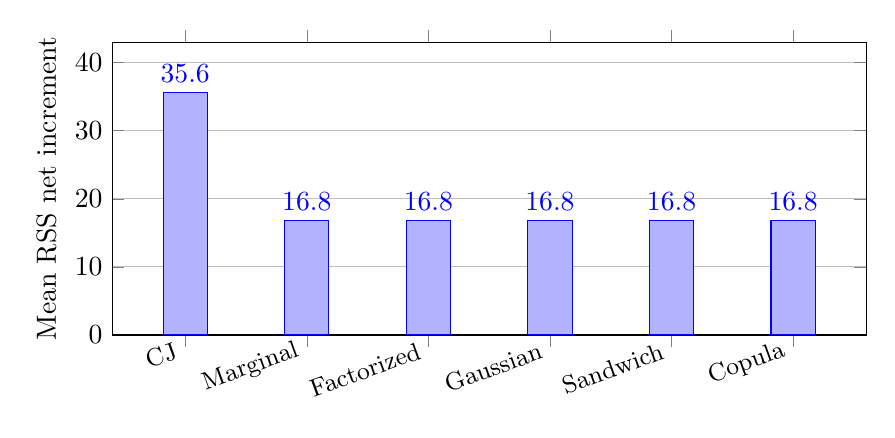
\begin{tikzpicture}
\begin{axis}[ybar,bar width=16pt,width=.92\linewidth,height=5.3cm,
symbolic x coords={CJ,Marginal,Factorized,Gaussian,Sandwich,Copula},xtick=data,
x tick label style={font=\small,rotate=20,anchor=east},
ylabel={Mean RSS net increment},ymin=0,ymax=43,
enlarge x limits=.12,ymajorgrids=true,nodes near coords]
\addplot coordinates {(CJ,35.6) (Marginal,16.8) (Factorized,16.8)
(Gaussian,16.8) (Sandwich,16.8) (Copula,16.8)};
\end{axis}
\end{tikzpicture}
\caption{Complete paid utility within the matched conditional-fusion
family, at identical fixed reservation and loss budget. Four additional
beneficial leases provide the CJ increment. This is development evidence;
the stronger legacy operational policies and new physical validation
are retained separately.}
\label{fig:conditional-rss-return}
\end{figure}

\subsection{Joint information controls useful actions at fixed summaries}
\label{sec:rss-pairing-bridge}
We execute the retained-law bridge in
Proposition~\ref{prop:retained-pairing-paid-bridge} at
$\tau\in\{0,0.25,0.5,0.75,1\}$. All three paths use exactly the
frozen CJ source forecasts, matured history, quality, bandwidth and issued
$q_k$ sequence. The first preserves every coordinate mixture marginal;
the second also removes off-diagonal correction covariance from the paired
endpoint; the third preserves the complete residual mean and covariance.
The mixture is formed before target-line normalization, including its
current-disagreement evidence. No controller is selected from this grid.

Table~\ref{tab:rss-pairing-bridge} retains all 15 operating levels.
The full endpoint has the largest paid return and beneficial-action count
on every displayed path. Its return is at least that of every other level
in each of the five individual delay replays. All levels retain the nine
baseline beneficial leases; every changed action relative to $\tau=0$
is beneficial. The common harmful lease and two zero-return leases remain,
so the measured increment is entirely additional useful deployment.
The full fixed-mean/covariance path is particularly informative: mean
return increases from 16.8 to 24.4, 28.8 and 35.6 at
$\tau=0.5,0.75,1$, while the full second-order residual summary stays
unchanged. Retained distributional shape therefore contributes an executed
paid gain that those summaries cannot reproduce in this controlled family.

\begin{table}[t]
\centering\small
\caption{All frozen-state RSS information interventions under the same
Fixed130/$B=130$ execution rule. Each entry is mean net increment /
pooled beneficial admissions. Columns vary retained pairing only.
Every level retains one harmful admission and two zero-return admissions.}
\label{tab:rss-pairing-bridge}
\resizebox{\linewidth}{!}{%
\begin{tabular}{lrrrrr}
\toprule
Preserved information & $\tau=0$ & $0.25$ & $0.5$ & $0.75$ & $1$\\
\midrule
Fixed marginals & 16.8 / 9 & 16.8 / 9 & 16.8 / 9 & 34.4 / 12 & 35.6 / 13\\
Fixed marginals; diagonal $P$ & 16.8 / 9 & 16.8 / 9 & 16.8 / 9 & 28.8 / 11 & 35.6 / 13\\
Fixed full mean/covariance & 16.8 / 9 & 16.8 / 9 & 24.4 / 10 & 28.8 / 11 & 35.6 / 13\\
\bottomrule
\end{tabular}}
\end{table}

With fixed full mean/covariance, $\tau=0.5$ recovers the $+38$ lease;
$\tau=0.75$ additionally recovers $+22$; the full endpoint also recovers
$+6$ and $+28$. With fixed coordinate marginals, $\tau=0.75$ recovers
$+22,+38,+28$, and $\tau=1$ adds $+6$. These are complete paid returns,
not changes in predicted scores alone. The same diagonal-$P$ endpoint
retains the four actions, connecting the benefit to historical pairing.
The unguarded full endpoint identifies a fifth $+19$ opportunity, which the
primary budget refuses; full guarded extra return remains 94, matching the
locked-policy comparison exactly.

At seed 88002, origin 164, the full-mean/covariance bridge gives paid
scores $(-0.556835,-0.263031,0.033936,0.334119,0.637568)$ at the five
retained-law fractions. At $\tau=0.5$ the conditional paired-law mass is
0.494636, agreeing with the evidence-weighted bridge. The endpoints change
$F$ from 4.637708 to 5.833289 and $S$ from 38.908502 to 39.144119,
at the identical issued $q=0.005$. The exact score change is
$(5.833289-4.637708)-0.005(39.144119-38.908502)=1.194403$.
It crosses the paid threshold and executes a $+38$ lease while preserving
the full residual mean and covariance. This case directly links retained
distributional shape, conditional target correction, issued action and
complete return.

\begin{figure}[t]
\centering
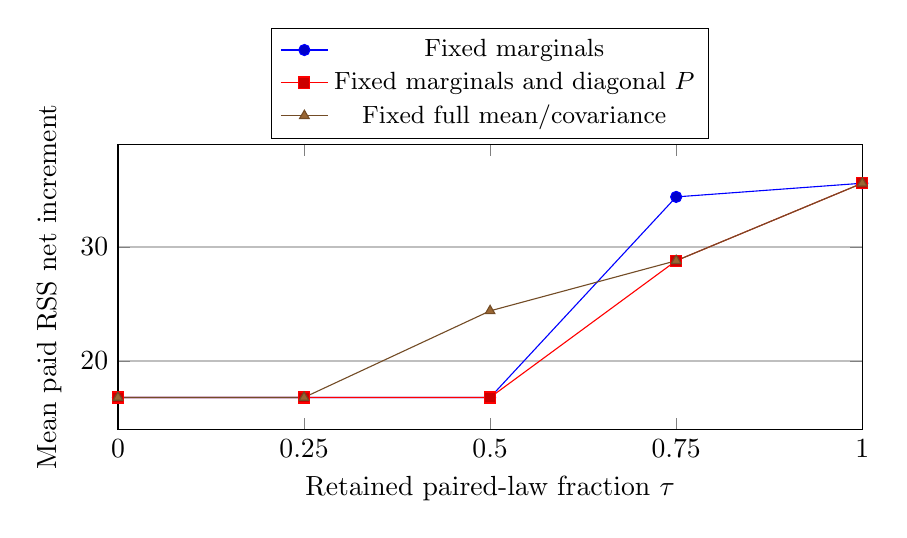
\begin{tikzpicture}
\begin{axis}[width=.91\linewidth,height=5.2cm,
xmin=0,xmax=1,xtick={0,.25,.5,.75,1},ymin=14,ymax=39,
xlabel={Retained paired-law fraction $\tau$},
ylabel={Mean paid RSS net increment},ymajorgrids=true,
legend style={at={(.5,1.02)},anchor=south,legend columns=1,font=\small}]
\addplot+[mark=*] coordinates {(0,16.8) (.25,16.8) (.5,16.8) (.75,34.4) (1,35.6)};
\addplot+[mark=square*] coordinates {(0,16.8) (.25,16.8) (.5,16.8) (.75,28.8) (1,35.6)};
\addplot+[mark=triangle*] coordinates {(0,16.8) (.25,16.8) (.5,24.4) (.75,28.8) (1,35.6)};
\legend{Fixed marginals,Fixed marginals and diagonal $P$,Fixed full mean/covariance}
\end{axis}
\end{tikzpicture}
\caption{Restoring joint information changes executed paid return while
specified source summaries remain fixed. Lines connect only the five
measured intervention levels. The issued calibration sequence is held at
CJ's causal values; the paths are mechanism replays on known RSS,
not separately trained policies or independent physical replications.}
\label{fig:rss-pairing-bridge}
\end{figure}

These interventions preserve the issued CJ calibration sequence to isolate
information effects. Independently calibrated complete policies remain in
Table~\ref{tab:conditional-development}, and broader operational choices
remain in Table~\ref{tab:operational-comparison}. At the full endpoint,
all posterior moments and actions reproduce the frozen CJ record.
Across 210 states and 3,150 issued numerical scores, endpoint moment error
is at most $2.64\times10^{-16}$; complete service reconstruction error is
zero. The full-mean/covariance identity agrees within
$5.55\times10^{-17}$ and the diagonal-$P$ coordinate variance identity
within $6.94\times10^{-18}$. The archive retains every score, evidence
ratio, issued threshold, changed action, guarded trajectory and numerical
refinement, including unchanged levels.

\subsection{Actual admission calibration and active budget constraints}
Table~\ref{tab:conditional-admission-calibration} reports all RSS admitted
coverage and optimistic excess. CJ has 11/16 covered admitted targets,
versus 8/12 for the exact-marginal, factorized and copula controls and
5/12 for Gaussian and sandwich. Its covered fraction increases by
2.08 percentage points over the exact marginal and 27.08 over Gaussian;
the denominator and severity columns are necessary because the admitted
sets differ. Mean admitted optimistic excess is 2.611 units for CJ,
3.337 for the exact marginal, 3.650 for Gaussian and 4.016 for copula.
These are observed action-related improvements on RSS, rather than
nominal 90\% coverage guarantees.

\begin{table}[t]
\centering\small
\caption{RSS coverage and excess at actually executed admissions under
$B=130$. Excess is $S_k(T_k-q_k)_+$ in complete-return units. Fractions,
sums and maxima retain the full calibration evidence.}
\label{tab:conditional-admission-calibration}
\begin{tabular}{lrrrr}
\toprule
Controller & Covered / admitted & Excess sum & Excess mean & Excess max\\
\midrule
CJ & 11/16 & 41.768 & 2.611 & 11.777\\
Exact marginal & 8/12 & 40.040 & 3.337 & 10.804\\
Factorized & 8/12 & 35.788 & 2.982 & 9.533\\
Full Gaussian / GLS & 5/12 & 43.795 & 3.650 & 10.940\\
Block sandwich & 5/12 & 46.116 & 3.843 & 11.238\\
Gaussian copula & 8/12 & 48.193 & 4.016 & 13.162\\
CJ--diagonal $P$ & 11/16 & 41.699 & 2.606 & 11.734\\
\bottomrule
\end{tabular}
\end{table}

GasHome has five beneficial CJ leases totaling 226 units, 5/5 admitted
coverage and zero optimistic excess, matching the conditional controls.
AReM has five harmful leases totaling $-150$ and 0/5 admitted coverage
for every conditional method; per-schedule charged loss is at most 31,
below the 130-unit budget. These development outcomes distinguish the
pathwise safety theorem from correct calibration and profitable updating.
The retained first selector and its stronger-smoothing revision are labeled
development iterations; they do not become independent physical validation.

The declared budget grid is $B\in\{0,110,130,260\}$ with fixed reserve
130. Budgets zero and 110 admit no fixed-reserve lease. On RSS, CJ has
mean unguarded increment 39.4, versus 35.6 at $B=130$: one positive
$+19$ lease is refused following the settled $-1$ loss. At $B=260$,
the extra valid reservation is feasible and the mean returns to 39.4.
The primary policy remains $B=130$. The outcome demonstrates actual
budget activation, including its opportunity cost; positive gains never
refund permanent spent loss. Every recorded spent-loss-plus-reserve and
service-prefix bound agrees with Eq.~\eqref{eq:pathwise-loss-budget}.

\subsection{Information-geometry evidence and paid policy comparisons}
The original precision-norm controller G is distinct from CJ. Its original
eight tasks are Occupancy, Room, MHEALTH, smartphone HAR, Gas Sensor
Array Drift, DSADS, HAR70+ and RSS
\cite{occupancy357,occupancy864,mhealth319,har240,gas224,dsads256,har780,rss348}.
G has no harmful complete lease in those original reported tasks.
It obtains mean reference-relative gains 218.8 on Gas Drift, 2.0 on
DSADS and 30.2 on RSS, and ties on the other five tasks. These statements
apply to that executed version and evidence set, rather than extending
its zero-harm result to subsequent algorithms or AReM.

On RSS, G and scalar-information admission each execute ten pooled leases.
G retains nine beneficial leases and no harmful one; scalar information
retains seven beneficial leases and one harmful one. Two additional $+38$
leases and one avoided $-1$ lease give $(76+1)/5=15.4$ mean extra utility.
G's admitted coverage is 6/10 versus 4/10; optimistic excess totals are
3.7189 versus 12.6217. At seed 88003, origin 164, holding correction
mean, predictive risk, source quality and issued threshold fixed changes
the gate from $+3.7825$ to $-1.6884$ when non-scalar precision geometry
is replaced by scalar mass. G admits an actual $+38$ lease. The stored
forecasts, executed model, served requests, closure and restoration allow
the entire information--action--return chain to be reconstructed.

\begin{figure}[t]
\centering
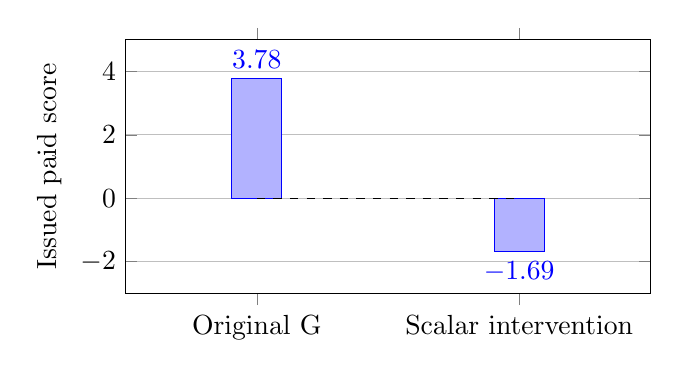
\begin{tikzpicture}
\begin{axis}[ybar,bar width=18pt,width=.68\linewidth,height=4.8cm,
symbolic x coords={Original G,Scalar intervention},xtick=data,
ylabel={Issued paid score},ymin=-3,ymax=5,enlarge x limits=.5,
ymajorgrids=true,nodes near coords]
\addplot coordinates {(Original G,3.7825) (Scalar intervention,-1.6884)};
\draw[dashed] (axis cs:Original G,0)--(axis cs:Scalar intervention,0);
\end{axis}
\end{tikzpicture}
\caption{The preserved RSS $+38$ information-geometry action. This is an
actual fixed-state intervention on original G, whose versions and numerical
records are retained; it is not relabeled as a CJ posterior action.}
\label{fig:preserved-rss-geometry}
\end{figure}

Stronger prior operational choices and published-method adaptations are
also relevant. Table~\ref{tab:operational-comparison} retains their RSS
paid results under the same guard. Conditional-law controls in
Table~\ref{tab:conditional-controls} isolate retained joint information;
these operational alternatives assess the broader service choice. The
legacy factorized and sandwich policies obtain higher RSS utility than CJ.
Thus the new pairing gain within matched conditional inference does not
establish that CJ is the best available operational controller.

\begin{table}[t]
\centering\small
\caption{RSS operational comparisons at fixed reserve 130 and $B=130$.
Earlier frozen-policy and external runs are retained in the dependency
archives; they use the same complete paid service accounting. Counts pool
five delay schedules and distinguish beneficial from harmful leases.}
\label{tab:operational-comparison}
\begin{tabular}{lrrrr}
\toprule
Policy & Mean net increment & Admitted & Beneficial & Harmful\\
\midrule
CJ & 35.6 & 16 & 13 & 1\\
Original G & 30.2 & 10 & 9 & 0\\
Legacy factorized precision policy & 44.8 & 14 & 13 & 0\\
Legacy block-sandwich policy & 44.4 & 18 & 15 & 1\\
PDF, nonlinear active objectives & 35.2 & 19 & 15 & 3\\
QMF, nonlinear active objectives & 15.0 & 15 & 9 & 4\\
PDF, linear active objectives & 9.0 & 11 & 6 & 4\\
QMF, linear active objectives & 19.4 & 12 & 8 & 3\\
SAEF, published-rule adaptation & 19.6 & 13 & 9 & 3\\
\bottomrule
\end{tabular}
\end{table}

\subsection{Frozen validation on a new four-source physical collection}
Before acquisition we froze all scientific code, information controls,
fees, budgets, seed schedules and tuning grids for UCI Localization Data
for Person Activity (196) \cite{localization196}. The collection contains
five people, five recordings per person and four actual localization tags:
left ankle, right ankle, chest and belt. A/B fit prefix models, C calibrates,
and D/E supply the held-out recordings. Every C, D and E recording is a
separate service chain, resetting prefix models, training buffer, error
archive, initial quantile and loss budget. No lease, lag, model adaptation
or statistical callback crosses a recording or participant boundary.

Causal preparation keeps chest events 0,2,4,\ldots before freshness
filtering, joins each tag's latest available event no later than the
anchor, and requires calendar age between zero and one second.
Coordinates and observed age give 16 physical features; current and two
recording-reset lags plus an intercept give 49 model inputs. Normalization
and quality use only hash-separated prefix fitting/error records. All
11 original activity classes are retained. The official metadata describes
unique numeric timestamps, but one E04 pair is tied; before fitting we
amended only this parser assertion and retained both raw events using
(timestamp, original-row) order. The original acquisition freeze, amended
metadata bindings and unchanged scientific-source hashes are preserved.

\begin{table}[t]
\centering\small
\caption{Actual causal records in the new physical validation. Prefix
fitting and held-out error records are disjoint. All five recordings per
person remain; test rows are not used for selection.}
\label{tab:new-physical-data}
\begin{tabular}{lrrr}
\toprule
Role / people & Recordings & Retained rows & Complete test origins\\
\midrule
Prefix A/B & 10 & 6,664 (4,700 fit; 1,964 error) & --\\
Calibration C & 5 & 3,839 & --\\
Test D & 5 & 3,278 & 24\\
Test E & 5 & 4,010 & 29\\
\bottomrule
\end{tabular}
\end{table}

The 164,860 raw rows yield 17,791 causally aligned rows; 117 stride-selected
anchors are excluded by freshness. An independent label-blind reconstruction
checks every retained anchor, source raw row, source feature and age, and
all 60 feature-history runs. The one tied right-ankle event follows the
chest event in original order and is unavailable at that anchor.
No future-nearest join, interpolation or label-dependent alignment is used.

Each arm has 27 calibration-schedule evaluations, or 135 actual C-recording
chain evaluations. All internal second-half calibration returns are zero;
the predeclared tie rule selects $b=1$ and $q_{\min}=q_0=1.2815515655$.
PDF and QMF select learning rate 0.02 and margin zero, with initial
quantiles 1.43183 and 1.52827, respectively. All nine selections are locked
together before testing. Test seeds are 113001--113005; calibration seeds
are 112001--112003. All outcomes remain separate from controller selection.

\begin{table}[t]
\centering\small
\caption{Frozen held-out physical outcomes. Values sum the five separately
reset recording chains for a person and average five shared delay schedules.
Every internal and external method retains the reference. No admitted
coverage estimate exists when no lease executes.}
\label{tab:new-physical-results}
\begin{tabular}{lrrrr}
\toprule
Method & D mean net / increment & E mean net / increment & Admissions & Harmful\\
\midrule
CJ & 2266.6 / 0 & 2482.6 / 0 & 0 & 0\\
Exact marginal & 2266.6 / 0 & 2482.6 / 0 & 0 & 0\\
Factorized & 2266.6 / 0 & 2482.6 / 0 & 0 & 0\\
Full Gaussian / GLS & 2266.6 / 0 & 2482.6 / 0 & 0 & 0\\
Block sandwich & 2266.6 / 0 & 2482.6 / 0 & 0 & 0\\
Gaussian copula & 2266.6 / 0 & 2482.6 / 0 & 0 & 0\\
CJ--diagonal $P$ & 2266.6 / 0 & 2482.6 / 0 & 0 & 0\\
PDF, nonlinear active objectives & 2266.6 / 0 & 2482.6 / 0 & 0 & 0\\
QMF, nonlinear active objectives & 2266.6 / 0 & 2482.6 / 0 & 0 & 0\\
\bottomrule
\end{tabular}
\end{table}

CJ covers 262/265 issued targets (98.87\%) and 76/78 informative targets
(97.44\%); admitted coverage is undefined, 0/0. Informative origins have
nonzero current candidate/reference disagreement, defined before outcome
labels. Issued optimistic excess totals 8.293 units, maximum 4.684;
informative excess totals 5.173. These high issued fractions accompany
complete abstention and cannot demonstrate improved calibration at useful
executed decisions. D has no positive complete fork; E has ten positive
counterfactual episodes totaling 98 units across the five delays, all missed
by every controller. The seven CJ point forecasts above paid cost are
still rejected: its maximum forecast is 9.272, minimum scale 10.745,
minimum $q$ is 1.28155 and maximum issued paid score is $-10.316$.
Same-joint-state interventions produce no admission difference.

Budgets zero, 110, 130 and 260 all have zero spent loss, zero reservation
and zero refused proposals in this validation. Thus the safety guarantee
is respected but does not actively constrain a paid update here.
The 450 selected policy trajectories and 1,800 budget trajectories have
zero service-reconstruction discrepancy; all current-truth poisoning and
historical-label-maturity checks pass. Maximum target-integral moment
refinement error is $3.83\times10^{-11}$, separate from copula-CDF
approximation error. These are implementation checks, not 450 independent
physical replications. There is one new collection and two held-out people;
the five delays reuse each recorded physical stream.

\subsection{Final-algorithm validation on unseen dual-sensor participants}
\label{sec:harth-frozen-validation}
The final original-CJ numerical method, all information controls, service
fees, reserves, budgets, source groups, participant roles and tuning grids
were bound before acquisition of HARTH \cite{harth779}. This collection
contains two simultaneous physical accelerometers on the lower back and
right front thigh. We retain all 22 participants, ordered by numeric
original identifier: eight fit the prefix, four calibrate, and ten supply
the held-out evaluation. None of the ten test participants occurs in either
fitting or calibration. The algorithm was selected on known development
traces, rather than on HARTH outcomes.

Each physical source supplies its three acceleration coordinates. We
retain raw acquisition rows $0,50,100,\ldots$ at the documented 50-Hz
sampling rate, producing direct nominal 1-Hz snapshots without an
anti-alias filter. Current and two previous retained observations give
nine coordinates per source and 18 joint coordinates, plus an intercept.
All 12 original activity classes remain. Normalization and source models
use only the first 70\% of each fitting participant; the remaining 30\%
forms the prefix error/prior set. Causal histories reset at participant
boundaries and every raw timestamp gap exceeding one second. No lease,
lag, adaptation, error archive or calibration callback crosses such a gap.

\begin{table}[t]
\centering\small
\caption{Actual HARTH data retained by the frozen label-independent stride.
History runs are service-reset segments within participants; they are not
additional independent people or sites.}
\label{tab:harth-data}
\begin{tabular}{lrrr}
\toprule
Role & Participants & Retained rows & History runs\\
\midrule
Prefix fitting/error & 8 & 57,407 & 253\\
Calibration & 4 & 26,847 & 134\\
Held-out test & 10 & 44,982 & 195\\
\bottomrule
\end{tabular}
\end{table}

The 6,461,328 raw rows yield 129,236 retained records. Both sensor views
come from exactly the same acquisition row and timestamp. A pre-fitting
decoder amendment accepts the official files' inert export index in
S015/S021 and unnamed export index in S023; it preserves the eight
scientific columns, row values, row ordering, stride and participant roles.
The original acquisition binding, prior decoder, failure record and amendment
are retained. The declared diagonal-$P$ dispatch had also been restored
before acquisition, with its prior source snapshot preserved.
All numerical fusion, fitting and service functions stayed
unchanged; this representation repair did not use a model or test result.

The primary setting is a fixed 130-unit reserve with a permanent 130-unit
loss budget for each actual history run. Diagnostic budgets are
$0,110,130,260$. Every internal arm receives nine configurations and three
shared calibration delays, seeds 122001--122003. Selection maximizes pooled
second-half guarded net return; the predeclared tie rule favors the larger
floor and bandwidth, or the smaller prior standard deviation for a legacy
arm. Each published neural objective receives nine learning-rate/margin
configurations on the same four calibration participants. Its unchanged
helper calibrates all fully matured issued origins, including unready
origins, whereas internal calibration uses ready origins. This denominator
difference is retained explicitly. All eleven selections, trained external
prefix models, cache and scientific source hashes are locked together
before held-out replay. Test seeds 123001--123005 reuse the same ten
physical participants under five imposed feedback schedules.

The evaluated conditional arms all select bandwidth one, floor zero and
initial quantile zero; their delayed causal updates remain active. The
legacy factorized controller selects prior standard deviation 0.2 and
floor 0.64, and the legacy sandwich selects 0.2 and floor zero. These are
calibration selections, not test-based changes. We aggregate service return
over each participant's runs before averaging schedules. Participant
comparisons and paired delay comparisons are kept separate. Because the
ledger resets at every history run, the aggregate pathwise bound per
schedule is $195B$, rather than $B$ or $10B$.


\subsection{Held-out useful actions, paid return and strong comparisons}
\label{sec:harth-outcomes}
The frozen CJ controller produces mean reference-relative net return 48.2
on the ten held-out participants. The five schedule totals are
$[49,13,111,27,41]$, with conditional $t_4$ descriptive interval
$[1.39,95.01]$. Ten of its twelve admitted leases are beneficial, one has
zero return and one loses 11 units. The ten beneficial replay admissions
occur at four distinct participant/run/origin opportunities, on S021,
S024, S026 and S029; delay schedules do not turn them into ten independent
physical opportunities. Their pooled positive return is 252, giving
$(252-11)/5=48.2$ after complete service interruptions and fees.
This is new useful-deployment evidence from participants unused in fitting,
calibration or algorithm development.

\begin{table}[t]
\centering\small
\caption{All frozen HARTH controllers under fixed reserve 130 and
$B=130$ per history run. Mean increment first sums all ten participants
within a delay schedule. Action counts and negative loss pool all five
schedules. Coverage uses the issued threshold at actual admissions.
NN denotes the declared nonlinear adaptation of the published objective.}
\label{tab:harth-net}
\resizebox{\linewidth}{!}{%
\begin{tabular}{lrrrrrrr}
\toprule
Controller & Mean $\Delta J$ & Admitted & Beneficial & Harmful & Zero
 & Negative loss & Admitted coverage\\
\midrule
CJ & 48.2 & 12 & 10 & 1 & 1 & 11 & 9/12\\
Exact marginal & 117.2 & 16 & 14 & 1 & 1 & 11 & 13/16\\
Factorized & 116.2 & 17 & 14 & 2 & 1 & 16 & 13/17\\
Full Gaussian / GLS & 48.2 & 12 & 10 & 1 & 1 & 11 & 9/12\\
Block sandwich & 43.2 & 12 & 9 & 2 & 1 & 21 & 8/12\\
CJ--diagonal $P$ & 48.2 & 12 & 10 & 1 & 1 & 11 & 9/12\\
Gaussian copula & 48.2 & 12 & 10 & 1 & 1 & 11 & 9/12\\
Legacy factorized precision & 93.6 & 6 & 6 & 0 & 0 & 0 & 6/6\\
Legacy block sandwich & 119.4 & 21 & 15 & 4 & 2 & 9 & 14/21\\
PDF, active objectives, NN & 876.0 & 111 & 96 & 13 & 2 & 72 & 59/111\\
QMF, active objectives, NN & 883.4 & 109 & 96 & 11 & 2 & 58 & 48/109\\
\bottomrule
\end{tabular}}
\end{table}

Participant-level aggregation exposes where the useful actions occur.
CJ's schedule-averaged increments for S020--S029 are
$[0,0.4,0,0,12.2,0,16.0,0,0,19.6]$.
The mean per participant is 4.82; the ten-person $t_9$ descriptive
dispersion interval is $[-0.81,10.45]$. It is distinct from the
conditional delay interval and does not assert a random sample of sites.
The remaining six participants have no CJ deployment.

\begin{figure}[t]
\centering
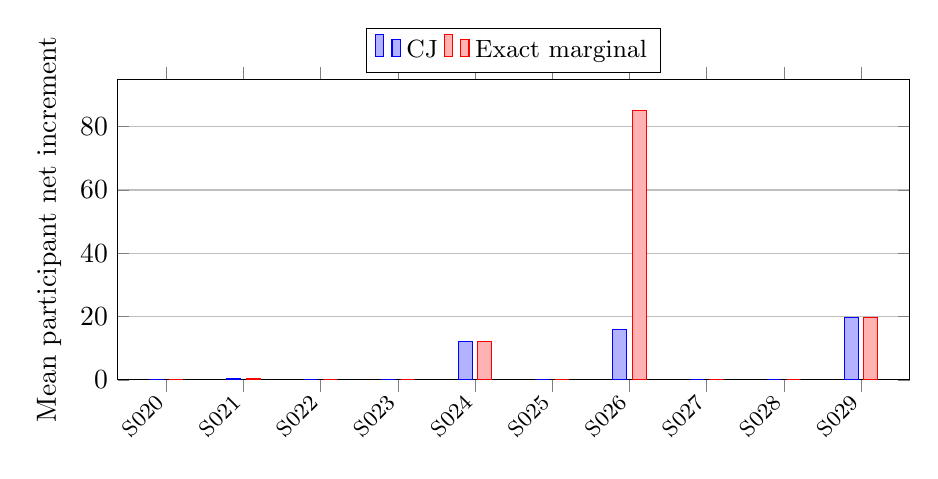
\begin{tikzpicture}
\begin{axis}[ybar,bar width=5pt,width=.96\linewidth,height=5.4cm,
symbolic x coords={S020,S021,S022,S023,S024,S025,S026,S027,S028,S029},
xtick=data,x tick label style={rotate=45,anchor=east,font=\footnotesize},
ylabel={Mean participant net increment},ymin=0,ymax=95,
enlarge x limits=.07,ymajorgrids=true,
legend style={at={(.5,1.02)},anchor=south,legend columns=2,font=\small}]
\addplot coordinates {(S020,0) (S021,.4) (S022,0) (S023,0) (S024,12.2)
 (S025,0) (S026,16) (S027,0) (S028,0) (S029,19.6)};
\addplot coordinates {(S020,0) (S021,.4) (S022,0) (S023,0) (S024,12.2)
 (S025,0) (S026,85) (S027,0) (S028,0) (S029,19.6)};
\legend{CJ,Exact marginal}
\end{axis}
\end{tikzpicture}
\caption{Every held-out HARTH participant, aggregated over its history
runs and averaged over the same five delays. Four physical participants
provide CJ useful-deployment evidence. The largest difference from the
exact-marginal control is concentrated in S026; other participants tie.}
\label{fig:harth-participants}
\end{figure}

The complete changed-action decomposition in
Eq.~\eqref{eq:action-gain-decomposition} measures independent operational
gain without equating fewer updates with better service.
Table~\ref{tab:harth-changed-actions} retains every comparator. Against
the matched block-sandwich control, CJ adds one $+15$ action and avoids
one $-10$ action, with no missed benefit or additional loss:
$(15+10)/5=5.0$ mean gain. The paired-delay interval is
$[-3.78,13.78]$; the mean participant difference is 0.5 with descriptive
interval $[-0.27,1.27]$. Two participants improve and eight tie.

\begin{table}[t]
\centering\small
\caption{Exact pooled CJ-minus-control action return on HARTH.
The first four numerical columns are nonnegative return magnitudes.
Their signed sum divided by five gives the final mean difference.
Methods sharing every CJ action are grouped only in this decomposition.}
\label{tab:harth-changed-actions}
\resizebox{\linewidth}{!}{%
\begin{tabular}{lrrrrr}
\toprule
Comparator & Additional gain & Avoided loss & Missed gain
 & Incurred loss & Mean difference\\
\midrule
Gaussian / copula / diagonal $P$ & 0 & 0 & 0 & 0 & 0\\
Exact marginal & 0 & 0 & 345 & 0 & $-69.0$\\
Factorized & 0 & 5 & 345 & 0 & $-68.0$\\
Block sandwich & 15 & 10 & 0 & 0 & 5.0\\
Legacy factorized precision & 129 & 0 & 345 & 11 & $-45.4$\\
Legacy block sandwich & 0 & 9 & 354 & 11 & $-71.2$\\
PDF, active objectives, NN & 132 & 72 & 4,332 & 11 & $-827.8$\\
QMF, active objectives, NN & 106 & 58 & 4,329 & 11 & $-835.2$\\
\bottomrule
\end{tabular}}
\end{table}

Both matched matrix and stronger operational comparisons matter.
The exact-marginal control admits four additional beneficial replays of
one S026 physical opportunity, whose returns sum to 345. Its mean exceeds
CJ by 69.0. The factorized control also incurs an additional five-unit
loss, giving CJ-minus-factorized return $-68.0$. Full Gaussian, copula
and diagonal-$P$ controls have exactly the same executed actions as CJ.
Consequently, this held-out collection establishes positive CJ deployment
and a gain over one adaptive matrix control, but does not replicate RSS's
gain from joint shape beyond the full covariance.

The external PDF/QMF comparisons activate their published training
objectives and retain all calibrated pipelines, rather than treating a
fixed confidence formula as a complete original method. On HARTH both
select learning rate 0.2, margin four and initial quantile zero.
Their larger mean returns, 876.0 and 883.4, accompany 96 beneficial
replay admissions each and higher pooled negative losses of 72 and 58.
They use two nonlinear source encoders rather than CJ's linear source
classifiers, and their helper includes unready issued origins in quantile
calibration. These disclosed differences make the external results
full-pipeline comparisons; the matched internal controls isolate retained
fusion information. Equal search counts and a common execution bound do
not turn differing backbones or calibration denominators into identical
fusion-only conditions.

\paragraph{Two complete conditional-law action chains.}
At S024/run0009, window 68, seed 123005, CJ issues
$F=5.269596$, $S=25.560318$ and $q=0$, hence
$L=+0.269596$. The matched sandwich issues $F=4.926124$ and
$L=-0.073876$. CJ admits; gross contrast 19, one lost correct request
and three fee units produce $D=19-1-3=+15$.
This crossing is a target-mean effect because $q=0$. Full Gaussian and
exact marginal also admit it, so it is not uniquely attributable to
non-Gaussian pairing.
At S026/run0005, window 68, seed 123002, CJ has
$F=6.053936$, $S=15.457619$, $q=0.075$ and $L=-0.105385$.
The sandwich has $F=6.080614$, $S=12.754443$ and $L=+0.124031$.
CJ rejects a complete $D=-10$ lease. The independent service
reconstruction verifies the two paid outcomes and their 25-unit pooled
advantage, while the full-Gaussian and exact-marginal controls make the
same decisions at these two origins.

\subsection{Decision calibration and an active execution-bound check}
\label{sec:harth-calibration}
CJ covers 1,418/1,560 issued targets (90.90\%), 215/289 informative
targets (74.39\%), and 228/325 information-ready targets (70.15\%).
Coverage at actual admission is 9/12 (75\%), below the nominal 90\%.
Optimistic admitted excess
$E_k=S_k(T_k-q_k)_+$ has total 15.9152, mean 1.3263 and maximum
11.1018 units. These are complete-return quantities entering
Eq.~\eqref{eq:weighted-return-bound}, not standardized scores alone.
The positive $+2$ action, the $-11$ action and the zero-return action
are uncovered. A beneficial outcome therefore does not itself establish
coverage of the issued conservative target.

\begin{table}[t]
\centering\small
\caption{Optimistic excess at actual HARTH admissions. All controllers
use the same conservative complete-service target; coverage denominators
appear in Table~\ref{tab:harth-net}. Values pool five shared delays.}
\label{tab:harth-admitted-excess}
\begin{tabular}{lrrr}
\toprule
Controller & Total excess & Mean per admission & Maximum\\
\midrule
CJ & 15.9152 & 1.3263 & 11.1018\\
Exact marginal & 15.9240 & 0.9952 & 11.1025\\
Factorized & 21.8674 & 1.2863 & 11.1025\\
Full Gaussian / GLS & 15.9229 & 1.3269 & 11.1232\\
Block sandwich & 26.0895 & 2.1741 & 11.2462\\
CJ--diagonal $P$ & 15.9152 & 1.3263 & 11.1018\\
Gaussian copula & 15.9234 & 1.3270 & 11.1023\\
Legacy factorized precision & 0 & 0 & 0\\
Legacy block sandwich & 33.0334 & 1.5730 & 11.2496\\
PDF, active objectives, NN & 768.1860 & 6.9206 & 35.0972\\
QMF, active objectives, NN & 992.9444 & 9.1096 & 62.3239\\
\bottomrule
\end{tabular}
\end{table}

The matched sandwich's admitted coverage is 8/12 and excess is 26.0895;
CJ improves both in this comparison. The exact-marginal control covers
13/16 admissions and the legacy factorized controller 6/6. Coverage and
excess are evaluated alongside utility, since declining costly updates can
reduce exposure without establishing a generally calibrated posterior.
The RSS pairing evidence, HARTH useful deployments and HARTH calibration
answer separate empirical questions.

\begin{table}[t]
\centering\small
\caption{CJ budget interventions with its frozen posterior and delayed
gate. Negative loss and refusal counts pool five delays; maximum loss is
over an individual history-run/schedule ledger. A fixed reserve of 130
necessarily blocks every positive proposal when $B<130$.}
\label{tab:harth-budgets}
\begin{tabular}{rrrrrr}
\toprule
$B$ & Mean $\Delta J$ & Admissions & Refused & Negative loss
 & Maximum chain loss\\
\midrule
0 & 0 & 0 & 12 & 0 & 0\\
110 & 0 & 0 & 12 & 0 & 0\\
130 & 48.2 & 12 & 0 & 11 & 11\\
260 & 48.2 & 12 & 0 & 11 & 11\\
\bottomrule
\end{tabular}
\end{table}

The lower-budget checks make reservation binding in eleven run/schedule
ledgers and reject twelve proposals before service. At the primary budget,
CJ's largest chain loss is 11 and its minimum service-prefix increment is
$-10$, within the valid reserve; no CJ proposal is budget-refused.
PDF and QMF each have three budget-refused proposals at $B=130$.
All controllers satisfy the same pathwise bound over all 42,900 budget
trajectories. Budget enforcement is thus demonstrated separately from
positive return and admitted calibration; it is not assigned exclusively
to joint fusion.

\paragraph{Source closure, exact execution reuse and reconstruction.}
All 28 operative scientific-source hashes and the shared eleven-controller
selection lock are checked before testing. The shared lock SHA-256 begins
\texttt{3b8840f72ff5ac40}; the raw HARTH archive begins
\texttt{2ab54d6b11467ddb}; the lossless processed cache begins
\texttt{4217c2a7c0c7dbcc}. A separately bound execution wrapper reuses only
byte-identical supplied-model twenty-step neural training calls on buffers
larger than the 512-row online buffer. Complete input/model hashes and deep
copies protect the cache; prefix-only tests verify exact cold/miss/hit
model and work equality and mutation/RNG isolation. The uncached partial
calibration attempt and its interruption record are retained. Cached
calibration reruns the complete unchanged grid, and every selection is
locked afterwards. This optimization changes execution time, not the
fusion rule, model updates or evaluation choices; the portable launcher
uses the original uncached training by default.

Request-level service reconstruction agrees exactly for internal runs;
the external maximum discrepancy is $1.42\times10^{-14}$. Complete-target
identity error is at most $2.84\times10^{-14}$, and the minimum numerical
slack in the return bound is $-7.11\times10^{-15}$. Current-truth poisoning
passes 14,040 internal checks. An independent completed-record verifier
checks all 195 test-run inventories, 10,725 selected policy trajectories,
42,900 budget trajectories, 1,560 fixed CJ states and 14,960 matured
callbacks. It reconstructs reservations, atomic settlements, chronological
quantiles, admitted coverage, excess and the four-term changed-action
identity. These trajectory counts establish implementation consistency;
physical generalization evidence remains ten people in one collection.

\subsection{Recent discounted-belief fusion under the paid service contract}
\label{sec:dbf2025-service}
We add Discounted Belief Fusion (DBF), published at AISTATS 2025
\cite{dbf2025}, and evidence averaging (EAvg) with the same evidence input.
This is a separately frozen benchmark extension on the already inspected
RSS and HARTH collections. It leaves the original CJ selections and all
physical evaluation results unchanged. DBF and EAvg receive the identical
linear source forecasts, prefix quality, physical masks, candidate/reference
versions, delayed complete feedback, common model work and paid service
ledger. The comparison implements the published DBF fusion operator with
an explicit evidence adapter; it does not reproduce its original evidential
backbone training.

For available source $s$, class count $K$ and prefix mean quality $\bar q$,
the common adapter uses $e_s=\kappa(q_s/\bar q)p_s$,
$\alpha_s=e_s+\mathbf1$, concentration $A_s=\sum_c\alpha_{s,c}$,
belief $b_s=e_s/A_s$, uncertainty $u_s=K/A_s$ and mean
$r_s=\alpha_s/A_s$. The author-code rule with conflict exponent one is
\begin{equation}
\begin{aligned}
 c_{st}&=\tfrac12\|r_s-r_t\|_1(1-u_s)(1-u_t),\qquad
 \eta_s=\prod_t(1-c_{st}-10^{-6}),\\
 b'_s&=\eta_sb_s,\qquad u'_s=1-\eta_s+\eta_su_s,\\
 e_{\rm DBF}&=m^{-1}\sum_s\frac{K b'_s}{u'_s+10^{-6}},\qquad
 p_{\rm DBF}=\frac{e_{\rm DBF}+\mathbf1}{\sum_c(e_{{\rm DBF},c}+1)}.
\end{aligned}
\label{eq:dbf-service-adaptation}
\end{equation}
The product includes self-comparison, as in the cited author implementation.
EAvg uses $e_{\rm EAvg}=m^{-1}\sum_se_s$ and the same Dirichlet mean.
Consequently, EAvg isolates conflict discounting from the common adapter's
quality weighting and shrinkage. Adapted evidence is declared input,
rather than evidence recovered from an original evidential network.

Both rules fit their own scalar complete-error correction with the existing
context kernel and historical targets, and receive calibrated paid admission.
Each evaluates nine configurations,
$\kappa\in\{K/4,K,4K\}$ crossed with margins $\{0,4,12\}$, on the same
three calibration delays. Only matured first-half errors fit the initial
90th quantile; second-half guarded return selects the configuration. The
unchanged external helper includes unready origins in this quantile and
its callbacks, while CJ's initial calibration requires ready origins.
This difference is recorded explicitly. Both tasks' selections and the
analysis script are hash-locked before any secondary test replay.
RSS selects $\kappa=8$, margin zero and initial quantiles 0.0029221
and 0.0003672 for DBF and EAvg, respectively. HARTH selects $\kappa=48$,
margin zero and initial quantile zero for both. Their initial quantile
denominators are 60 on RSS (51 ready, nine unready) and 176 on HARTH
(69 ready, 107 unready).

\begin{table}[t]
\centering\small
\caption{All selected recent-rule adaptations at fixed reserve 130 and
$B=130$ per chain. Mean net increment averages five shared delays; counts
and negative-loss magnitudes pool them. CJ rows are the unchanged archived
physical results. The DBF/EAvg scalar helper permits prior-only origins.}
\label{tab:dbf2025-complete-service}
\begin{tabular}{llrrrrr}
\toprule
Task & Controller & Mean $\Delta J$ & Beneficial & Harmful
 & Negative loss & Admitted coverage\\
\midrule
RSS & CJ & 35.6 & 13 & 1 & 1 & 11/16\\
RSS & DBF operator & 16.2 & 6 & 3 & 10 & 6/10\\
RSS & EAvg & 19.4 & 8 & 3 & 10 & 7/12\\
HARTH & CJ & 48.2 & 10 & 1 & 11 & 9/12\\
HARTH & DBF operator & 654.4 & 59 & 7 & 54 & 59/67\\
HARTH & EAvg & 664.8 & 62 & 12 & 102 & 61/75\\
\bottomrule
\end{tabular}
\end{table}

On RSS, CJ increases mean paid utility by 19.4 relative to DBF and by
16.2 relative to EAvg. It produces 13 beneficial admissions versus six
and eight, and reduces pooled negative loss from ten to one unit.
The exact CJ-minus-DBF action accounting is
$(129+10-41-1)/5=19.4$; against EAvg it is
$(129+10-57-1)/5=16.2$. The paired conditional delay intervals are
$[-33.84,72.64]$ and $[-43.36,75.76]$, respectively. These comparisons
extend the measured RSS benefit to a recent published fusion rule under
the common paid contract, while Table~\ref{tab:rss-four-extra-leases}
isolates joint-information value at an identical issued threshold.

On HARTH, 44 DBF admissions have no matured eligible historical evidence
and contribute 544.2 mean units; EAvg has 49 such admissions contributing
556.0. The remaining ready admissions contribute 110.2 and 108.8,
respectively, before intervening on the ledger. CJ requires information
readiness. Thus Table~\ref{tab:dbf2025-complete-service} compares complete
adapted pipelines with a disclosed readiness/calibration difference; it
does not isolate the DBF conflict operator against CJ's joint target law.
The complete HARTH CJ-minus-DBF and CJ-minus-EAvg means are $-606.2$
and $-616.6$. DBF versus EAvg has identical evidence, gate and tuning:
its conflict discount avoids 48 units of loss but misses 100 units of
benefit on HARTH, for $(48-100)/5=-10.4$ mean difference.
All additional, missed, avoided and incurred returns are retained.

\paragraph{Locked-score readiness alignment.}
After the primary extension, a separate bound diagnostic requires matured
eligible error evidence for DBF/EAvg admission. It changes only readiness,
keeps the selected evidence concentration, margin and every issued
$F,S,q$ fixed, and reconstructs all ledger events from the original
unguarded proposals. Outcomes are not obtained by subtracting prior-only
returns from a saved total. The selected calibration return becomes 4.333
for both rules on HARTH, without reselection; RSS selections and test actions
are unchanged. The protocol was bound before this diagnostic replay,
with SHA-256 beginning \texttt{be0d66cba05e4eeb}.

\begin{table}[t]
\centering\small
\caption{Locked-score HARTH readiness diagnostic at the same fixed-130
reservation and per-run loss budget. Existing parameters, forecasts and
calibration trajectories are retained. These are known-data interventions;
the quantile-fitting denominators remain those of the original pipelines.}
\label{tab:dbf2025-ready-alignment}
\begin{tabular}{lrrrrr}
\toprule
Controller & Mean $\Delta J$ & Admitted & Beneficial
 & Negative loss & Admitted coverage\\
\midrule
CJ, archived & 48.2 & 12 & 10 & 11 & 9/12\\
DBF, require ready evidence & 110.2 & 23 & 15 & 54 & 15/23\\
EAvg, require ready evidence & 108.8 & 26 & 16 & 63 & 15/26\\
\bottomrule
\end{tabular}
\end{table}

The complete CJ-minus-DBF accounting becomes
$(2+54-355-11)/5=-62.0$; against EAvg it becomes
$(0+63-355-11)/5=-60.6$. DBF's ready-only advantage over EAvg is
$(9-2)/5=1.4$. This separates the large prior-only admission effect from
the remaining evidence-fusion and scalar-target effects. Equal readiness
and execution guarantees do not equalize the archived quantile denominators
or the retained error representation. The matched marginal/matrix
comparisons, with CJ's target construction and calibration protocol,
remain the direct joint-information comparisons.

The extension checks source-order permutation, opinion normalization,
zero evidence, singleton evidence and an independent scalar implementation
of the author rule. The maximum scalar-versus-vector difference is
$1.11\times10^{-16}$. Request-level service, fork, delayed-feedback and
budget reconstruction accompany all selected trajectories and all four
budgets $0,110,130,260$. The protocol SHA-256 begins
\texttt{6e08d55dde6e2b0b}; the analysis was bound before secondary replay.

\subsection{Theory-to-execution verification and reproducibility}
The parity construction in Eq.~\eqref{eq:conditional-parity-laws} is checked
under feasible history age weights, actual outage eligibility and complete
service targets, not only unconstrained abstract atoms. Thirty-two
full-source origins from the last 48 eligible opportunities at current
origin 240 have eight examples per pattern. Label-free context attenuation
and disagreement support $126/128$ give effective mass 1.5 per pattern
under $\beta=0.97$. The declared prior, masked state, smoothing and
$q=1.2815515655$ yield paired scores $-18.212062$ and $+1.069772$;
exact-marginal scores are $-15.266708$ in both regimes and full-Gaussian
scores are $-9.980616$ in both. The admitted $+12$ lease has independently
reconstructed service return $+12$ and minimum service-prefix increment
$-2$, within its identical reserve. The harmful regime is rejected.
Implementation and independent posterior moments agree within
$8.33\times10^{-17}$, and current-truth poisoning leaves the forecasts
unchanged. Full finite generative enumeration verifies expected information
value gap $6/43$; it is a model construction, not a physical-task statistic.
Exact rational evaluation over 1,032 generative outcomes further checks
Proposition~\ref{prop:final-fitted-paid-benefit} for 50 fitted gates against
four reduced-information policies per case, including common-feasibility
restrictions. This verifies the bridge from the information gap to the
fitted paid action and its estimation-error and admission-penalty terms.

The supplied \texttt{Fusion\_Conditional\_Target\_Repro} package retains
all scientific sources, old and revised development selectors, every
calibration trial, selected configurations, complete actions and callbacks,
mask and data provenance, numerical proofs, independent analyzers and new
physical replay records. The previous frozen packages remain unchanged
dependencies. From the extracted package directory, run:
\begin{verbatim}
python run_reproduction.py verify
python run_reproduction.py theory --output /absolute/new/empty/theory
python run_reproduction.py physical --output /absolute/new/empty/replay
\end{verbatim}
The accompanying \texttt{Fusion\_RSS\_Pairing\_Evidence} supplement retains
all 15 fixed-state information paths, lossless numerical inputs, all 3,150
scores, complete guarded records, an independent four-action extraction and
the bridge proof checks. A NumPy-only cached-state replay runs from its root:
\begin{verbatim}
python verify_cached.py
python run_proof_checks.py --output /absolute/new/empty/proof
\end{verbatim}
The first command independently regenerates target moments, scores,
proposals and fixed-reserve returns from 210 frozen states. Its cached-state
scope is distinct from raw-request reconstruction, which uses the unchanged
physical engines and provenance archive. The second command checks the
posterior-bridge identities and score perturbation inequalities; it produces
synthetic proof checks rather than new physical outcomes.

The portable launcher writes to an empty external directory and preserves
delivered records. Only filesystem bindings are rebased; numerical model,
estimation, posterior, gate and service functions stay byte-identical.
Full posterior states, issued rows, callbacks and guarded service trajectories
are compared, rather than checking total utility alone. Python 3.12.14 and
NumPy 2.3.5 suffice; no SciPy, PyTorch or scikit-learn is needed. UCI196's
CC BY 4.0 provenance, raw/archive hashes, metadata-only timestamp amendment,
all freeze phases and package hashes are included.

The final \texttt{Fusion\_CJ\_Frozen\_Physical\_Repro} package is
self-contained for HARTH. It preserves all 28 bound scientific source
files byte-for-byte, the full processed data cache, every calibration trial,
all eleven selections, both test pipelines, all budget interventions and
the independent completed-record verifier. Prior source snapshots, parser
amendments, acquisition records and the unused CJ-R/CJ-T/CJ-Q development
candidates are retained. Those candidates were assessed on already known
RSS and were not promoted; HARTH does not select a replacement algorithm.
From this package's root, the commands are:
\begin{verbatim}
python run_reproduction.py verify
python run_reproduction.py theory --output /absolute/new/theory
python run_reproduction.py physical-calibrate --output /absolute/new/replay
python run_reproduction.py external-calibrate --output /absolute/new/replay
python run_reproduction.py locktest --output /absolute/new/replay
python run_reproduction.py physical-test --output /absolute/new/replay
python run_reproduction.py external-test --output /absolute/new/replay
python run_reproduction.py analyze --output /absolute/new/analysis
\end{verbatim}
The five calibration/lock/test phases share one new output directory and
run as separate processes. Analysis independently recomputes the archived
completed-record audit and all tables without retraining. The optional
\texttt{--cache-prefix-training} flag applies only to the two external
phases and records its separate execution audit. Scientific outputs are
compared with the delivered records: actions and discrete structure exactly,
numeric leaves to absolute tolerance $10^{-10}$ plus relative tolerance
$10^{-12}$. The output records also state exact decoded equality and the
observed maximum difference. HARTH's CC BY 4.0 attribution and all raw-file
hashes are included; the 310.8-MB official raw archive is not required for
the processed-cache replay. Replaying delivered test data establishes
reproducibility and does not constitute another unseen-data validation.

The \texttt{Fusion\_Coupling\_Focus\_Repro} supplement adds the paid-pairing
certificate, the continuous-density proof check and the complete DBF/EAvg
extension. It retains every primary and readiness-intervention outcome,
all calibration trials, original selections and source/data hashes.
From its root, the following commands verify the frozen closure and
regenerate the archived numerical analyses in fresh output directories:
\begin{verbatim}
python portable_dbf_launcher.py verify
python portable_dbf_launcher.py readiness-verify
python portable_dbf_launcher.py analyze-rss --out /absolute/new/dbf-rss
python portable_dbf_launcher.py analyze-harth --out /absolute/new/dbf-harth
\end{verbatim}
The README also gives readiness-analysis and full calibration/test replay
commands. Filesystem rebasing leaves numerical function bodies unchanged.
The paid-pairing validator regenerates every frozen bridge score and all
four changed-action certificates from its bundled byte-identical inputs.
The continuous-density check compares independent line quadrature with
analytic mixture moments to $2.78\times10^{-17}$. These checks distinguish
reproducibility, information identification and observed physical return.

The retained joint law has a verified information distinction, a realizable
strict paid-action separation and a reconstructed RSS useful-deployment
increment. The new fixed-summary paths preserve coordinate marginals or
complete residual mean/covariance while recovering extra paid actions;
four executed leases retain all baseline useful deployments and add 94 net
units after service interruption and fees. The source, posterior, issued
score, budget decision and actual return are recorded for every crossing.
The original G information-geometry case remains identifiable as separate
version evidence. The central contribution is the paid value of retained
complete-action pairing: current disagreement selects a conditional target
that residual marginals and second-order summaries need not identify;
the RSS interventions preserve these summaries while recovering beneficial
paid actions. HARTH supplies useful deployments on four held-out participants
and the reconstructed conditional-law gain over the matched sandwich.
The complete operational tables locate these effects within their measured
comparison scope. The common execution ledger supplies the pathwise loss
guarantee for every arm; additional useful deployments and complete paid
return measure the fusion increment under that identical guarantee.

\ifdefined\FusionMainDocument
\else
\begin{thebibliography}{99}
\bibitem{gibbs2021}
I. Gibbs, E. J. Cand{\`e}s, Adaptive conformal inference under distribution
shift, Advances in Neural Information Processing Systems 34 (2021).
\url{https://proceedings.neurips.cc/paper/2021/hash/0d441de75945e5acbc865406fc9a2559-Abstract.html}.
\bibitem{occupancy357}
L. Candanedo, Occupancy Detection, UCI Machine Learning Repository,
2016. \url{https://doi.org/10.24432/C5X01N}.
\bibitem{occupancy864}
A. Singh, A. Chaudhari, Room Occupancy Estimation, UCI Machine Learning
Repository, 2018. \url{https://doi.org/10.24432/C5P605}.
\bibitem{mhealth319}
O. Banos, R. Garcia, A. Saez, MHEALTH Dataset, UCI Machine Learning
Repository, 2014. \url{https://doi.org/10.24432/C5TW22}.
\bibitem{har240}
J. Reyes-Ortiz, D. Anguita, A. Ghio, L. Oneto, X. Parra, Human Activity
Recognition Using Smartphones, UCI Machine Learning Repository, 2013.
\url{https://doi.org/10.24432/C54S4K}.
\bibitem{gas224}
A. Vergara, Gas Sensor Array Drift Dataset, UCI Machine Learning
Repository, 2012. \url{https://doi.org/10.24432/C5RP6W}.
\bibitem{dsads256}
B. Barshan, K. Altun, Daily and Sports Activities, UCI Machine Learning
Repository, 2010. \url{https://doi.org/10.24432/C5C59F}.
\bibitem{pdf2024}
B. Cao, Y. Xia, Y. Ding, C. Zhang, Q. Hu, Predictive dynamic fusion,
Proceedings of the 41st International Conference on Machine Learning,
PMLR 235 (2024) 5608--5628.
\url{https://proceedings.mlr.press/v235/cao24c.html}.
\bibitem{qmf2023}
Q. Zhang, H. Wu, C. Zhang, Q. Hu, H. Fu, J. T. Zhou, X. Peng,
Provable dynamic fusion for low-quality multimodal data,
Proceedings of the 40th International Conference on Machine Learning,
PMLR 202 (2023) 41753--41769.
\url{https://proceedings.mlr.press/v202/zhang23ar.html}.
\bibitem{har780}
A. Logacjov, A. Ustad, HAR70+, UCI Machine Learning Repository (2023).
\url{https://doi.org/10.24432/C5CW3D}.
\bibitem{minka2000}
T. P. Minka, Bayesian linear regression, technical note
(1998, revised 2010). \url{https://tminka.github.io/papers/minka-linear.pdf}.
\bibitem{rss348}
D. Bacciu, P. Barsocchi, S. Chessa, C. Gallicchio, A. Micheli,
Indoor User Movement Prediction from RSS Data, UCI Machine Learning
Repository (2014). \url{https://doi.org/10.24432/C5761H}.
\bibitem{arem366}
F. Palumbo, C. Gallicchio, R. Pucci, A. Micheli,
Activity Recognition system based on Multisensor data fusion (AReM),
UCI Machine Learning Repository (2016).
\url{https://doi.org/10.24432/C5SS33}.
\bibitem{gashome362}
F. Huerta, R. Huerta, Gas sensors for home activity monitoring,
UCI Machine Learning Repository (2016).
\url{https://doi.org/10.24432/C5BS4F}.
\bibitem{koliander2022}
G. Koliander, Y. El-Laham, P. M. Djuri{\'c}, F. Hlawatsch,
Fusion of probability density functions, Proceedings of the IEEE
110(4) (2022) 404--453. \url{https://doi.org/10.1109/JPROC.2022.3154399}.
\bibitem{localization196}
V. Vidulin, M. Lustrek, B. Kaluza, R. Piltaver, J. Krivec,
Localization Data for Person Activity, UCI Machine Learning Repository
(2010). \url{https://doi.org/10.24432/C57G8X}.
\bibitem{harth779}
A. Logacjov, A. Kongsvold, K. Bach, H. B{\aa}rdstu and P. Mork,
HARTH [Dataset], UCI Machine Learning Repository,
\href{https://doi.org/10.24432/C5NC90}{doi:10.24432/C5NC90}.

\bibitem{blackwell1953}
D. Blackwell, Equivalent comparisons of experiments,
The Annals of Mathematical Statistics 24(2) (1953) 265--272.
\url{https://doi.org/10.1214/aoms/1177729032}.
\bibitem{dbf2025}
G. Bezirganyan, S. Sellami, L. Berti-Equille, S. Fournier,
Multimodal Learning with Uncertainty Quantification based on Discounted
Belief Fusion, Proceedings of the 28th International Conference on
Artificial Intelligence and Statistics, PMLR 258 (2025) 3142--3150.
\url{https://proceedings.mlr.press/v258/bezirganyan25a.html}.
\end{thebibliography}
\end{document}
\fi
